% !TEX program = pdflatex
%%
%% This is file `sample-acmtog.tex',
%% generated with the docstrip utility.
%%
%% The original source files were:
%%
%% samples.dtx  (with options: `all,journal,bibtex,acmtog')
%% 
%% IMPORTANT NOTICE:
%% 
%% For the copyright see the source file.
%% 
%% Any modified versions of this file must be renamed
%% with new filenames distinct from sample-acmtog.tex.
%% 
%% For distribution of the original source see the terms
%% for copying and modification in the file samples.dtx.
%% 
%% This generated file may be distributed as long as the
%% original source files, as listed above, are part of the
%% same distribution. (The sources need not necessarily be
%% in the same archive or directory.)
%%
%%
%% Commands for TeXCount
%TC:macro \cite [option:text,text]
%TC:macro \citep [option:text,text]
%TC:macro \citet [option:text,text]
%TC:envir table 0 1
%TC:envir table* 0 1
%TC:envir tabular [ignore] word
%TC:envir displaymath 0 word
%TC:envir math 0 word
%TC:envir comment 0 0
%%
%% The first command in your LaTeX source must be the \documentclass
%% command.
%%
%% For submission and review of your manuscript please change the
%% command to \documentclass[manuscript, screen, review]{acmart}.
%%
%% When submitting camera ready or to TAPS, please change the command
%% to \documentclass[sigconf]{acmart} or whichever template is required
%% for your publication.
%%
%%
\documentclass[acmtog, nonacm]{acmart}

% --- REMOVE ACM BOILERPLATE ---
\settopmatter{printacmref=false, printccs=false} 
\setcopyright{none}              
\renewcommand\footnotetextcopyrightpermission[1]{} 
\renewcommand{\shortauthors}{}   

\acmDOI{}
\acmISBN{}
\acmYear{}
\acmVolume{}
\acmNumber{}
\acmArticle{}

\citestyle{acmauthoryear}
% ------------------------------

%%
%% \BibTeX command to typeset BibTeX logo in the docs
\AtBeginDocument{%
  \providecommand\BibTeX{{%
    Bib\TeX}}}

%% Rights management information.  This information is sent to you
%% when you complete the rights form.  These commands have SAMPLE
%% values in them; it is your responsibility as an author to replace
%% the commands and values with those provided to you when you
%% complete the rights form.

% ADD THESE LINES TO HIDE BOILERPLATE
%%
%% end of the preamble, start of the body of the document source.


%%
%% These commands are for a JOURNAL article.

%%
%% Submission ID.
%% Use this when submitting an article to a sponsored event. You'll
%% receive a unique submission ID from the organizers
%% of the event, and this ID should be used as the parameter to this command.
%%\acmSubmissionID{123-A56-BU3}

%%
%% For managing citations, it is recommended to use bibliography
%% files in BibTeX format.
%%
%% You can then either use BibTeX with the ACM-Reference-Format style,
%% or BibLaTeX with the acmnumeric or acmauthoryear sytles, that include
%% support for advanced citation of software artefact from the
%% biblatex-software package, also separately available on CTAN.
%%
%% Look at the sample-*-biblatex.tex files for templates showcasing
%% the biblatex styles.
%%

%%
%% The majority of ACM publications use numbered citations and
%% references.  The command \citestyle{authoryear} switches to the
%% "author year" style.
%%
%% If you are preparing content for an event
%% sponsored by ACM SIGGRAPH, you must use the "author year" style of
%% citations and references.

\usepackage[utf8]{inputenc}
\usepackage[T1]{fontenc}
\usepackage{tabularx}
\usepackage{url}

% Nuclear balance killer: Force-override commands before they can even be used
\makeatletter
\def\balance{}
\def\nobalance{}
\def\pbalance{}
\def\nopbalance{}
\AtBeginDocument{%
  \let\oldbalance\balance \let\balance\relax
  \let\oldpbalance\pbalance \let\pbalance\relax
}
\makeatother

%

% Preamble
\usepackage{xurl} 
\hypersetup{breaklinks=true}

\begin{document}

%%
%% The "title" command has an optional parameter,
%% allowing the author to define a "short title" to be used in page headers.
\title{\textbf{An Econometric Taxonomy for Policy: Quantifying Structural Vulnerability via K-Means Clustering of Philippine Industries}}


\author{Gheann Christie Mediodia Cuevas}
\affiliation{%
  \institution{De La Salle University}
  \city{Manila}
  \country{Philippines}
}

\author{Precious Mae Mercado Divina}
\email{precious_divina@dlsu.edu.ph}
\affiliation{%
  \institution{De La Salle University}
  \city{Manila}
  \country{Philippines}
}

\author{Aaron Joshua Estacio Sison}
\affiliation{%
  \institution{De La Salle University}
  \city{Manila}
  \country{Philippines}
 }


%%
%% By default, the full list of authors will be used in the page
%% headers. Often, this list is too long, and will overlap
%% other information printed in the page headers. This command allows
%% the author to define a more concise list
%% of authors' names for this purpose.

%%
%% The abstract is a short summary of the work to be presented in the
%% article.
\begin{abstract}
The Philippine Standard Industrial Classification (PSIC) groups industries by product output, masking structural differences that determine economic resilience. This study constructs a data-driven taxonomy by applying K-Means clustering to the firm-size distributions of 228 three-digit PSIC industries, using establishment and employment data from the Philippine Statistics Authority (2021). Three engineered features, average firm size, SME density, and large-firm density, serve as the structural fingerprint for each industry. The optimal four-cluster solution, validated by the Elbow Method (WCSS) and Silhouette Coefficient (0.4946), segments the economy into four archetypes. The Survivalist archetype (avg. 10.36 employees, entropy \texorpdfstring{$H \approx 0.41$}{H is approximately 0.41}) dominates the landscape. The Middle (45.52), Transition (175.00), and Oligopoly (823.29) clusters complete the taxonomy. Shannon Entropy confirms that these archetypes represent distinct levels of structural diversity. A regression of pandemic-era business closures on Survivalist industry share yields \texorpdfstring{$r = 0.44$}{r = 0.44}, establishing that structural fragility predicts vulnerability to systemic shock. Regional mapping reveals compressed risk scores (0.93--0.95), indicating nationwide structural fragility. The taxonomy provides an empirical basis for replacing uniform MSME policy with archetype-specific interventions.
\end{abstract}

%%
%% The code below is generated by the tool at https://dl.acm.org/ccs.cfm.
%% Please copy and paste the code instead of the example below.
%%
\begin{CCSXML}
<ccs2012>
 <concept>
  <concept_id>10010405.10010455.10010461</concept_id>
  <concept_desc>Applied computing~Sociology</concept_desc>
  <concept_significance>500</concept_significance>
 </concept>
 <concept>
  <concept_id>10010147.10010257.10010258.10010260.10010271</concept_id>
  <concept_desc>Computing methodologies~Bayesian network models</concept_desc>
  <concept_significance>300</concept_significance>
 </concept>
</ccs2012>
\end{CCSXML}

\ccsdesc[500]{Applied computing~Sociology}
\ccsdesc[300]{Computing methodologies~K-Means Clustering}



%%
%% This command processes the author and affiliation and title
%% information and builds the first part of the formatted document.
\maketitle
\thispagestyle{empty}
\pagestyle{plain}

\section{Introduction}

Micro, small, and medium enterprises (MSMEs) are nominally the backbone of the Philippine economy, comprising 99.5\% of registered establishments and generating the majority of local employment \citep{dti2023, psa2023}. However, this statistical dominance masks a "hollowed-out" industrial structure, where a vast base of survivalist micro-enterprises lie, this is what is called a missing middle of dynamic MSMEs, and a disconnect from high-productivity global value chains \citep{worldbank2020}. While economic literature consistently identifies MSMEs as drivers of inclusive growth \citep{llanto2017}, the persistence of this "missing middle" in the Philippines suggests a fundamental failure in how the state views and regulates its industrial base.

The core of this failure lies in the Philippine Government's "one-size-fits-all" approach to industrial policy. Government programs routinely treat broad sectors, such as "Manufacturing" or "Retail" as homogenous groups, assuming that a micro-scale food processor shares the same growth constraints and risks as a large-scale electronics exporter. This logic is flawed. As \citet{wachs2022} argue, standard industrial classifications (like NAICS or the Philippine PSIC in our case) act as a "limiting condition" for analysis because they group firms based on what they make (product) rather than how they operate (energy, capital, and labor structure). By relying on these static labels, policymakers "mask differences" between heterogeneous industries, leading to inefficient resource allocation and untargeted interventions. For instance, a simple sari-sari store is grouped under the same policy as a large supermarket chain. Both have different needs and capability, but the PSIC classifies them as the same thing.

This study posits that the root of the problem is not merely policy implementation, but the classification system itself. Grounded in the economic framework,  Structure-Conduct-Performance (SCP) paradigm, this research argues that an industry's Structure (specifically its firm-size distribution) is a primary determinant of its Performance (resilience and vulnerability). The COVID-19 pandemic served as a brutal empirical validation of this view. The crisis did not affect "Manufacturing" uniformly, but it decimated industries with specific structural vulnerabilities, those reliant on physical proximity or dominated by fragile micro-firms while sparing others. \citet{nava2021} demonstrated this in the U.S. context, using unsupervised machine learning to reveal that standard industry codes failed to capture these divergent "structural DNA" traits until they were re-clustered based on performance data.

To transcend the limitations of the Philippine Standard Industrial Classification (PSIC), this paper employs a data science approach to construct a new, data-driven industrial taxonomy. Following the methodological precedents of \citet{karaca2018} in Turkey, who successfully clustered manufacturing sectors using only establishment and employment counts and \citet{wachs2022} in the energy sector, this study utilizes K-Means clustering to re-segment the Philippine economy. By ignoring the "product labels" of the PSIC and focusing purely on structural variables, this research aims to identify the true "economic fault lines" of the Philippines. This moves the discourse from a descriptive analysis of what industries exist, to a prescriptive analysis of which structural archetypes possess the resilience required for long-term development, explicitly operationalizing \citet{shutters2024}'s insight that economic structure constrains future transition pathways.

\subsection{General Objective}
The primary objective of this study is to construct a data-driven industrial taxonomy of the Philippine economy based on the firm-size distribution or what we would define as its (``structural DNA'') comprised of the 3-digit PSIC industries. By utilizing unsupervised machine learning, this research aims to quantify structural heterogeneity and demonstrate that an industry's structural dna is a superior predictor of economic resilience than its nominal product classification.

\subsection{Specific Objectives}
To achieve the general objective, this study executes the following specific aims:
\begin{itemize}
    \item \textbf{Quantify the structural resolution loss of traditional classifications.} Estimate the divergence between nominal 1-digit PSIC labels and actual firm-size distributions to demonstrate the extent to which aggregate industrial codes mask latent structural heterogeneity.
    \item \textbf{Construct a data-driven taxonomy via unsupervised learning.} Apply K-Means clustering to 3-digit industry data to mathematically segment the economy into distinct ``structural archetypes'' (e.g., Survivalist vs. Oligopolistic). This specifically targets the detection of deviations from Gibrat's Law and the quantification of the ``Missing Middle'' phenomenon within specific sectors.
    \item \textbf{Validate cluster distinctiveness using Information Theory.} Compute the Shannon Entropy for each derived cluster to rigorously confirm that identified archetypes represent fundamentally distinct levels of complexity and diversity, rather than stochastic statistical artifacts.
    \item \textbf{Test the Structure-Resilience correlation under the SCP Paradigm.} Model the relationship between the derived structural archetypes and pandemic-induced business cessation rates. This isolates whether specific structural configurations possess an intrinsic, quantifiable vulnerability to systemic shock.
    \item \textbf{Spatially map the distribution of structural vulnerability.} Project the constructed taxonomy onto regional economic datasets to visualize the geographic concentration of specific industrial structures, providing the empirical basis for targeted, structure-specific policy interventions.
\end{itemize}

\subsection{Primary Research Question (PRQ):}
To what extent does the traditional 1-digit PSIC classification mask structural heterogeneity at the granular level, and can a 3-digit K-Means taxonomy based on firm-size distributions provide a superior framework for identifying an industry's vulnerability to systemic shocks?

\subsection{Secondary Research Questions (SRQs):}
\begin{itemize}
    \item What are the established limitations of high-level industrial classifications (like PSIC) for economic analysis, and how does K-Means clustering, using firm-size features, provide a methodologically-sound alternative?
    \item What are the emergent, data-driven ``structural archetypes'' of the Philippine economy when 3-digit PSIC industries are clustered by their firm-size distribution features (Table 3 \& Table 5)?
    \item How does this new taxonomy's ability to identify ``vulnerability to shock'' compare to the traditional 1-digit PSIC sections, using sectoral business closure data (Table 9) as the measure of vulnerability?
    \item How are these new structural archetypes geographically distributed across Philippine regions (Table 2), and what targeted, heterogeneous policy interventions does the taxonomy suggest?
\end{itemize}


\section{Review of Related Literature}

\subsection{Theoretical Foundations: From Representative Agents to Structural Heterogeneity}
The classical Structure-Conduct-Performance (SCP) paradigm, formalized by \citet{mason1939} and systematized by \citet{bain1956}, posits that an industry's structure is the primary determinant of its firms' conduct and, ultimately, their economic performance. \citet{scherer1990} extended this framework into the modern theory of industrial organization, establishing that market structure variables, including firm-size distribution, concentration ratios, and barriers to entry, shape competitive conduct and aggregate outcomes. This framework provides the theoretical basis for industrial policy, as it implies that by understanding and shaping an industry's structure, policymakers can influence its outcomes in innovation, employment, and resilience.

Traditional industrial policy, particularly horizontal policy that applies a uniform approach to broad sectors like Manufacturing, relies on a simplified assumption of homogeneity. This ``representative firm'' model broadly aligns with the static distribution implied by Gibrat's Law \citep{samuels1965}, which assumes firm growth rates are random and independent of size. However, \citet{evans1987} and \citet{hall1987} demonstrated systematic departures from this law, finding that smaller firms grow faster but fail more frequently. \citet{sutton1997} provided theoretical foundations for why Gibrat's Law breaks down in concentrated industries. These departures expose the critical importance of firm-size distribution as a policy variable.

This study rejects this assumption. We argue that the distribution of firm sizes within an industry is the critical, defining variable. The Philippine economy's ``missing middle,'' where a few large firms coexist with a vast base of micro-enterprises but weak SMEs, directly contradicts the smooth log-normal distribution assumed by Gibrat's Law, thus exposing a dangerous misalignment between policy design and economic reality.

\subsection{The Missing Middle as a Source of Systemic Risk}
This structural gap is more than a productivity issue, but a source of systemic vulnerability. Evidence from behavioral and empirical finance demonstrates that firm size strongly determines access to credit and, in turn, a firm's ability to survive economic shocks.

Large firms typically secure committed liquidity through long-term, unsecured credit lines. In contrast, SMEs rely on discretionary financing, characterized by short-term maturities, high collateral requirements, and demandable clauses that give banks the right to recall loans at any time. These financing differences produce starkly different crisis responses. During the COVID-19 pandemic, large firms drew heavily on committed credit lines to secure liquidity, while SMEs saw their discretionary credit effectively frozen as banks tightened lending.

Because private financial data for unlisted MSMEs is generally unavailable, the literature establishes that firm size is the single strongest proxy for financial constraints \citep{beck2008}. \citet{hsieh2009} demonstrated that misallocation of resources across firms of different sizes accounts for substantial productivity losses in developing economies. \citet{laporta2014} further established that informality, the condition of most micro-enterprises, is associated with fundamentally different production functions rather than merely smaller-scale versions of formal firms. Therefore, identifying an industry's size structure is effectively mapping its aggregate financial vulnerability. When policymakers miss these structural differences, support measures fail to reach the vulnerable ``middle,'' causing employment-rich sectors to collapse and deepening the economic shock.

\subsection{Flawed Taxonomies}
This policy blindness stems from a critical analytical failure. The traditional tool for economic analysis, the high-level (1-digit) Philippine Standard Industrial Classification (PSIC), is too coarse to guide targeted policy. Scholars note that such high-level classifications are ``ambiguous and simplistic'' and inadequate for modern decision-making.

High-level classifications group industries solely by output (e.g., ``Manufacturing''), masking significant differences at finer levels of detail. They treat an industry dominated by thousands of labor-intensive micro-bakeries as identical to one dominated by a few capital-intensive car manufacturers. This obscuration of the ``missing middle'' leads to uniform policies that are structurally mismatched to the industries they intend to help.

\subsection{The Data-Driven Taxonomies}
To resolve this, recent studies propose replacing broad classifications with bottom-up, data-driven automatic taxonomies. Unsupervised machine learning, and K-Means clustering in particular, has been validated as a methodologically sound approach to creating these new classification systems.

These studies establish two key precedents. First, K-Means clustering is a viable method for sorting industries into new, more meaningful groups based on structural traits rather than product labels. Second, this analysis must be performed at a granular level (e.g., 3-digit or 6-digit industry codes) to capture the true underlying economic structure. Furthermore, recent advances in Economic Complexity \citep{hidalgo2021} utilize Information Theory metrics, such as Shannon Entropy, to quantify the diversity and sophistication of economic systems. This provides a necessary mathematical validation for structural diversity that goes beyond simple counting.

\citet{haltiwanger2013} and \citet{decker2014} extended this line of inquiry by demonstrating that firm dynamics, including entry rates, exit rates, and the age-size distribution, carry substantially more information about economic vitality than static sector labels. Their work on ``business dynamism'' provides additional theoretical motivation for constructing taxonomies based on structural characteristics rather than product classifications.

\subsection{Synthesis and Research Gap}
This study synthesizes three strands of literature:
\begin{itemize}
    \item \textbf{The Problem (Finance):} Firm-size distribution dictates financial behavior and vulnerability to systemic shocks.
    \item \textbf{The Analytical Failure (Policy):} Traditional 1-digit classifications are simplistic and mask this granular vulnerability.
    \item \textbf{The Method (Data Science):} K-Means clustering is a valid method to create new, granular industrial taxonomies.
\end{itemize}

The research gap lies at the intersection of these three streams. To date, no study has applied K-Means clustering to firm-size distributions to explicitly address the limitations of the PSIC framework in the Philippine context. Additionally, we extend \citet{karaca2018}'s approach by incorporating distributional indicators like firm-size concentration ratios and average firm size.

\subsection{The Limitations of RA 9501 and Asset-Based Classification}
Finally, it is critical to address the prevailing legal framework for MSMEs in the Philippines, the Magna Carta for MSMEs (RA 9501). Currently, the state classifies firms purely by total assets or employment counts. While administratively convenient, this approach ignores the industrial ecosystem in which a firm operates.

Under RA 9501, a small software firm (characterized by low assets but high resilience and scalability) is treated identically to a small bakery (low assets, low resilience, and low scalability). Structural clustering addresses this deficiency by grouping firms based on their ecosystem behavior and structural composition, rather than a static balance sheet metric. This study posits that policy interventions targeting ``structural archetypes'' will be more effective than those targeting arbitrary asset thresholds.


\section{Research Methodology}

\subsection{Research Design}
This study employed a quantitative, explanatory research design grounded in the Structure-Conduct-Performance (SCP) paradigm. The core hypothesis is that an industry's Structure (its firm-size distribution) is a primary determinant of its Performance (economic resilience and vulnerability to shock).

The methodology proceeds in two phases:

\begin{description}
    \item[\textbf{Phase 1: Taxonomic Construction.}] An unsupervised machine learning model (K-Means) is utilized to segment the Philippine economy. It created a new taxonomy by clustering industries based on their ``structural DNA'' (firm-size distribution) rather than their stated output (PSIC codes).
    
    \item[\textbf{Phase 2: Ex-post Validation and Application.}] The resulting taxonomy was employed as an analytical lens to test the central hypothesis. Cluster labels were mapped to national resilience data (firm closures) and regional data to challenge the ``one-size-fits-all'' policy framework. This directly addresses the limitations of official classifications (like PSIC) which, as noted by \citet{wachs2022}, ``mask differences'' and are a ``limiting condition'' for effective analysis.
\end{description}

\subsection{Data Acquisition and Preparation}

\subsubsection{Data Set}
The data for this study was sourced from the Philippine Statistics Authority's (PSA) 2021 Updating of the List of Establishments (ULE).

\begin{itemize}
    \item \textbf{Unit of Analysis:} The 3-digit PSIC industry group (e.g., 'C101' - Manufacture of bakery products).
    \item \textbf{Modeling Data:} Phase 1 construction utilized:
    \begin{itemize}
        \item PSA Table 3: Total Employment by 3-digit PSIC.
        \item PSA Table 5: Total Establishments by MSME Size and 3-digit PSIC.
    \end{itemize}
    \item \textbf{Validation Data:} Phase 2 analysis utilized:
    \begin{itemize}
        \item PSA Table 9: Closures by Industry Section.
        \item PSA Table 2: Industries by Region.
    \end{itemize}
\end{itemize}

\subsubsection{Data Preprocessing}
The consolidated 3-digit industry dataset underwent list-wise deletion to remove any industry with null values for key variables (Total Employment or Total Establishments). Outliers were identified via Z-score analysis to determine if they are legitimate structural extremities (e.g., B062 - Extraction of natural gas) or data artifacts.

\subsection{Feature Engineering and Variables}
To create a ``structural fingerprint'' for each 3-digit PSIC industry, the following three independent variables were engineered. This 3-feature model is designed to be statistically robust by avoiding the perfect collinearity ($p_1+p_2+p_3=1$) that would arise from including all size-density ratios.

\begin{itemize}
    \item \textbf{avg\_firm\_size (Proxy for Scale):}
    \begin{itemize}
        \item \textbf{Formula:} 
        \begin{equation}
             \frac{\text{Total Employment from Table 3}}{\text{Total Establishments from Table 5}}
        \end{equation}
        \item \textbf{Precedent:} Based on \citet{karaca2018}, who used ``number of local units and the number of employees.''
    \end{itemize}

    \item \textbf{sme\_density (Proxy for ``The Middle''):}
    \begin{itemize}
        \item \textbf{Formula:} 
        \begin{equation}
            \frac{\text{Small Estabs.} + \text{Medium Estabs.}}{\text{Total Estabs.}}
        \end{equation}
        \item \textbf{Interpretation:} This variable directly quantifies the ``Missing Middle.''
    \end{itemize}
    
    \item \textbf{large\_density (Proxy for Concentration):}
    \begin{itemize}
        \item \textbf{Formula:} 
        \begin{equation}
            \frac{\text{Large Estabs.}}{\text{Total Estabs.}}
        \end{equation}
        \item \textbf{Interpretation:} Measures the dominance of large, established firms.
    \end{itemize}
\end{itemize}

These features mathematically describe the shape of an industry's firm-size distribution. Under the steady-state conditions implied by Gibrat's Law, firm sizes would follow a smooth log-normal distribution \citep{sutton1997}. Our features were designed to identify and group industries whose size distributions deviate from this theoretical benchmark, exhibiting concentration at the extremes rather than the smooth continuum the law predicts. Such deviations are the structural signature of the ``Missing Middle.''

\subsection{Phase 1: Taxonomic Construction and Statistical Validation}

\subsubsection{Preprocessing}
A preliminary descriptive analysis, including a correlation matrix and distribution plots, were performed on the three engineered features. As a distance-based algorithm, K-Means is sensitive to feature scale. Therefore, all three features were standardized using the StandardScaler function from Python's scikit-learn library, transforming them to a mean of zero and a standard deviation of one.

\subsubsection{Model Selection}
The clustering algorithm selected is K-Means, a non-overlapping (hard) partitioning algorithm. This choice is methodologically deliberate as the research goal is to create a definitive taxonomy for policy use. Hard clusters (where an industry belongs to one, and only one, archetype) are more operationally actionable for targeted policy than probabilistic ``soft'' assignments \citep{nava2021}.

\subsubsection{Statistical Validation (\texorpdfstring{$k$}{k}-Selection)}
To ensure the taxonomy is mathematically robust and minimizes researcher bias, a dual-validation protocol was established to determine the optimal number of clusters ($k$). This approach mitigates the specific limitations of individual metrics by triangulating between variance explanation and cluster separation.

\begin{itemize}
    \item \textbf{Elbow Method:} The Within-Cluster Sum of Squares (WCSS) was calculated for a range of $k$ values (e.g., $k \in [2, 8]$). This measures the compactness of clusters. The objective is to identify the "elbow" or inflection point where the marginal gain in explained variance begins to diminish, identifying the point of diminishing returns for structural segmentation.
    \item \textbf{Silhouette Coefficient:} The mean Silhouette Score was calculated for the same range. This quantifies how distinct each cluster is from its neighbors (ranging from -1 to 1). A higher score generally indicates greater separation and mathematical definition .
\end{itemize}

It is recognized in clustering literature that these metrics may diverge. For instance, the silhouette scores often favor broad, binary separation (e.g., low $k$), while the Elbow method may reveal more granular substructures.
Given the research objective to uncover the "Missing Middle," this study established a priority rule where in the event of divergence between the two metrics, the selection will prioritize Structural Resolution (Elbow) over global separation (Silhouette).
A strictly Silhouette-maximized solution (often $k=2$) risks determining a simplistic binary classification ("Small" vs. "Large") that aggregates heterogeneous subgroups into a single cluster. This would reproduce the aggregation bias of the current PSIC system. Therefore, the final $k$ was selected based on the Elbow inflection point that maintains a positive Silhouette score, ensuring the taxonomy captures the latent heterogeneity required for targeted policy intervention rather than maximizing simple geometric distance.

\subsection{Phase 2: Economic Validation and Application}

\subsubsection{Economic Validation and Archetype Profiling}
To ensure the cluster interpretations are mathematically backed and not subjective, an ex-post validation was performed using Shannon Entropy ($H$).

\begin{itemize}
    \item \textbf{Theory:} Shannon Entropy, a core concept in information theory, is used here as a measure of ``structural diversity.''
    \item \textbf{Formula:} 
    \begin{equation}
        H = - \sum_{i=1}^{4} p_i \ln(p_i)
    \end{equation}
    Where $p_i$ is the proportion of establishments in each of the four size buckets (Micro, Small, Medium, Large). Following standard convention in information theory, the term $0 \ln(0)$ is defined as 0 by the limit $\lim_{p \to 0^+} p \ln(p) = 0$. In practice, size buckets with zero establishments are excluded from the summation. Of the 228 industries in the dataset, 59 (25.88\%) have at least one empty size bucket, primarily in the Medium and Large categories.

    \item \textbf{Interpretation:}
    \begin{itemize}
        \item \textbf{Low Entropy ($H \approx 0$):} A ``structural monoculture'' or collapsed structure. The industry is dominated by a single firm size (e.g., 99\% Micro).
        \item \textbf{High Entropy ($H > 1.0$):} A ``complex ecosystem.'' The industry has a healthy, diverse mix of all firm sizes.
    \end{itemize}
\end{itemize}

This entropy score provided the objective, as the mathematical basis for profiling the clusters. For example, a cluster with high micro\_density (from 3.3) and low $H$ (from 3.5.1) is mathematically validated as a ``Fragmented'' archetype.

\subsubsection{Resilience and Vulnerability Analysis}
The new cluster labels were aggregated to the 1-digit PSIC Section level and merged with data from PSA Table 9 (Closures by Industry Section). This tested the central hypothesis that firm failure rates correlate with our structural archetypes. This directly "operationalizes" the concept from \citet{shutters2024} that economic structure, not just sector, determines ``vulnerability to shock.''

Since the cluster taxonomy is constructed at the 3-digit PSIC level while closure data is available only at the 1-digit Section level, a weighted aggregation method was employed. 1-digit Sections were characterized by the dominant structural cluster (by employment share) contained within them to avoid the ecological fallacy of attributing group-level characteristics to specific industries.

\subsubsection{Regional Economic Analysis}
The cluster labels were then mapped using GEOPANDAS and a map of the Philippines in a regional json file from Faeldon's Github repository, and the PSA Table 2 (Industries by Region) to create a geographic distribution of the Philippines' industrial archetypes. This analysis quantified the structural-economic differences between regions (e.g., NCR vs. BARMM) and provided evidence for designing targeted, non-uniform national MSME policies.

\subsection{Justification of Method}
The selection of K-Means is a deliberate choice to create a definitive industrial taxonomy for policy application. K-Means, a `hard clustering' algorithm, assigns each 3-digit industry to one, and only one, distinct cluster. This was superior for our purpose than `soft clustering' models (like Gaussian Mixture Models) that \citet{nava2021} used, which would assign industries a probability of belonging to all clusters. For designing actionable, targeted policy, distinct `hard' boundaries (e.g., an industry is in the `Survivalist' group) are more operationally useful than a probabilistic gradient. The K-Means algorithm, combined with the empirical validation of $k$ via the Silhouette Coefficient and the structural validation via Shannon Entropy, provides the most robust and reproducible ``white box'' model for creating a new, interpretable industrial taxonomy.

\subsection{Ethical Considerations}
All data utilized was secondary, aggregated at the 3-digit industry level by the Philippine Statistics Authority. No personally identifiable information (PII) or firm-level proprietary data was accessed or stored. The primary ethical consideration relates to the interpretation and application of the findings. The profiling of clusters (e.g., as ``vulnerable'') was handled with care, ensuring that such labels are understood as descriptive analytics to target development aid and support, not as pejorative labels for penalizing or disinvesting from specific sectors. All code and methodologies was documented to ensure transparency and replicability.

\subsection{Software and Hardware Configuration}
The data analysis was conducted using Python 3.11.11 within a UV-managed virtual environment. Key libraries included Pandas for data manipulation, Scikit-learn for feature scaling (StandardScaler) and clustering (KMeans), Matplotlib and Seaborn for visualization, SciPy for statistical testing, and GeoPandas for geographic mapping. Regional boundary data were sourced from Faeldon's open-source GeoJSON repository of Philippine administrative boundaries (2023 PSGC). The analysis was performed on a desktop workstation with an Apple M4 processor and 16GB of unified memory. 

\section{Results and Discussion}

\subsection{Structural Heterogeneity and the ``Missing Middle'' (RQ1)}
The descriptive analysis of the Philippine industrial structure refutes the utility of aggregate means. It reveals a fractured system defined by Structural Dualism. The descriptive statistics exhibit a negative skewness ($-0.3329$) in micro-enterprise density and a platykurtic distribution (excess kurtosis $= -0.7420$). The mild negative skew indicates a left-tail pull from industries with lower micro-density, while the platykurtic profile reflects a flatter-than-normal distribution rather than the peaked concentration Gibrat's Law would predict. Combined with the visual evidence in Figure \ref{fig:micro_density}, this profile is consistent with the ``Missing Middle'' hypothesis. The economy is not a smooth continuum of firm sizes as predicted by Gibrat's Law. It is a bimodal system polarized between a vast base of micro-entities and a thin layer of conglomerates.

\begin{figure}[ht]
    \centering
    \Description{A histogram showing the frequency distribution of micro-enterprise density across different industries. Most industries are clustered above the 90 percent threshold, indicating high structural fragility.}
    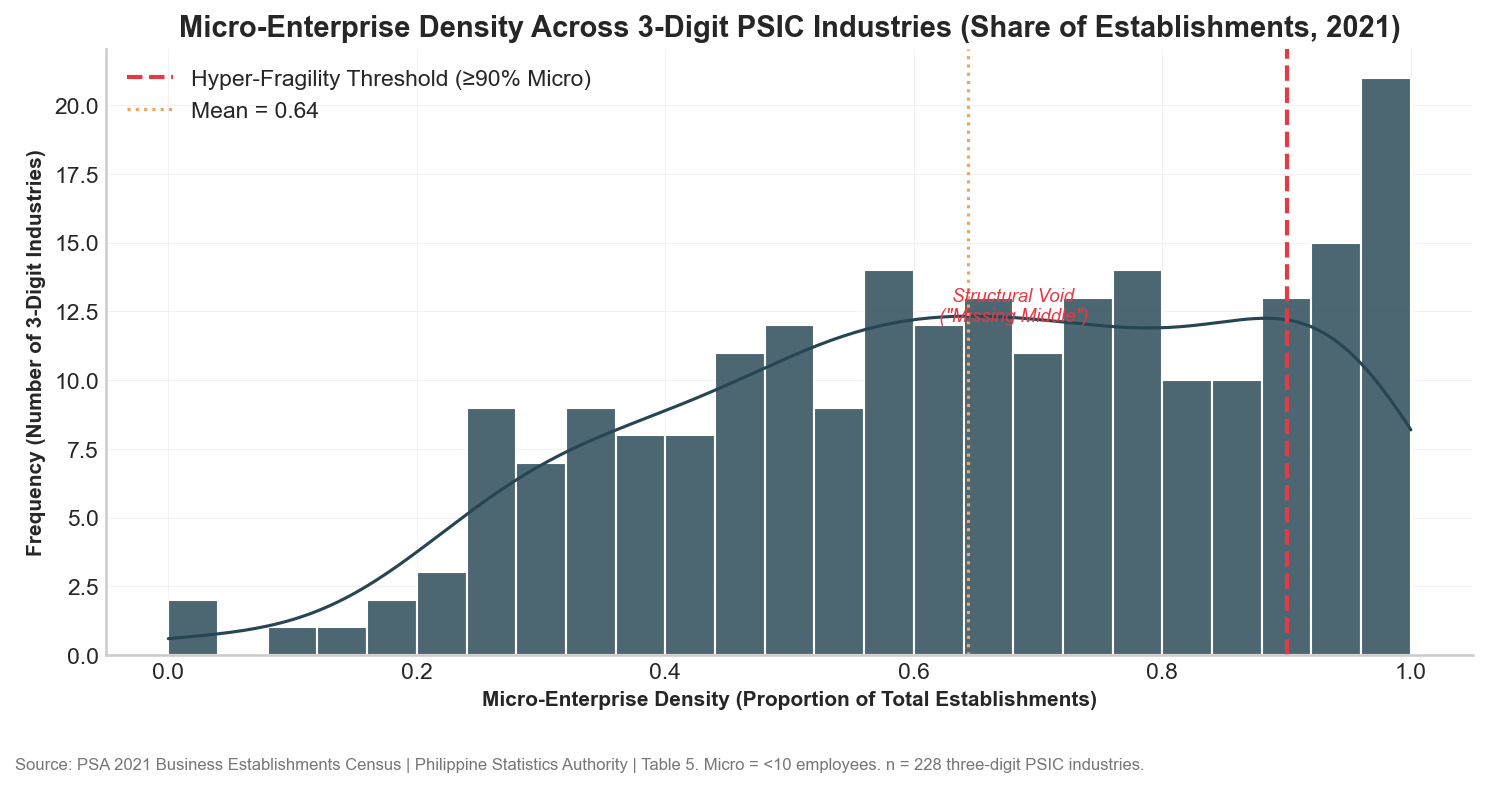
\includegraphics[width=1\linewidth]{fig_micro_density_histogram.png}
    \caption{Distribution of Micro-Enterprise Density Across Industries}
    \label{fig:micro_density}
\end{figure}

The distribution of micro-enterprise density across industries illustrates this structural void. As shown in Figure \ref{fig:micro_density}, the frequency distribution deviates from a standard Gaussian curve and shows a heavy concentration of industries above the 90\% ``Hyper-Fragility Threshold.'' This proves that the standard 1-digit PSIC classification masks extreme heterogeneity. While the ``Manufacturing'' sector is policy-treated as a monolith, our Z-score analysis ($Z > 3$) identifies structural outliers such as Manufacture of Electronic Components (C261) with an average firm size of 918.99. This bears no structural resemblance to the industry mean of 60.88.


\begin{figure}[ht]
    \centering
    \Description{A Pareto distribution of micro-enterprise counts across Philippine provinces, showing a high concentration of firms in a few urban hubs and a sparse distribution elsewhere.}
    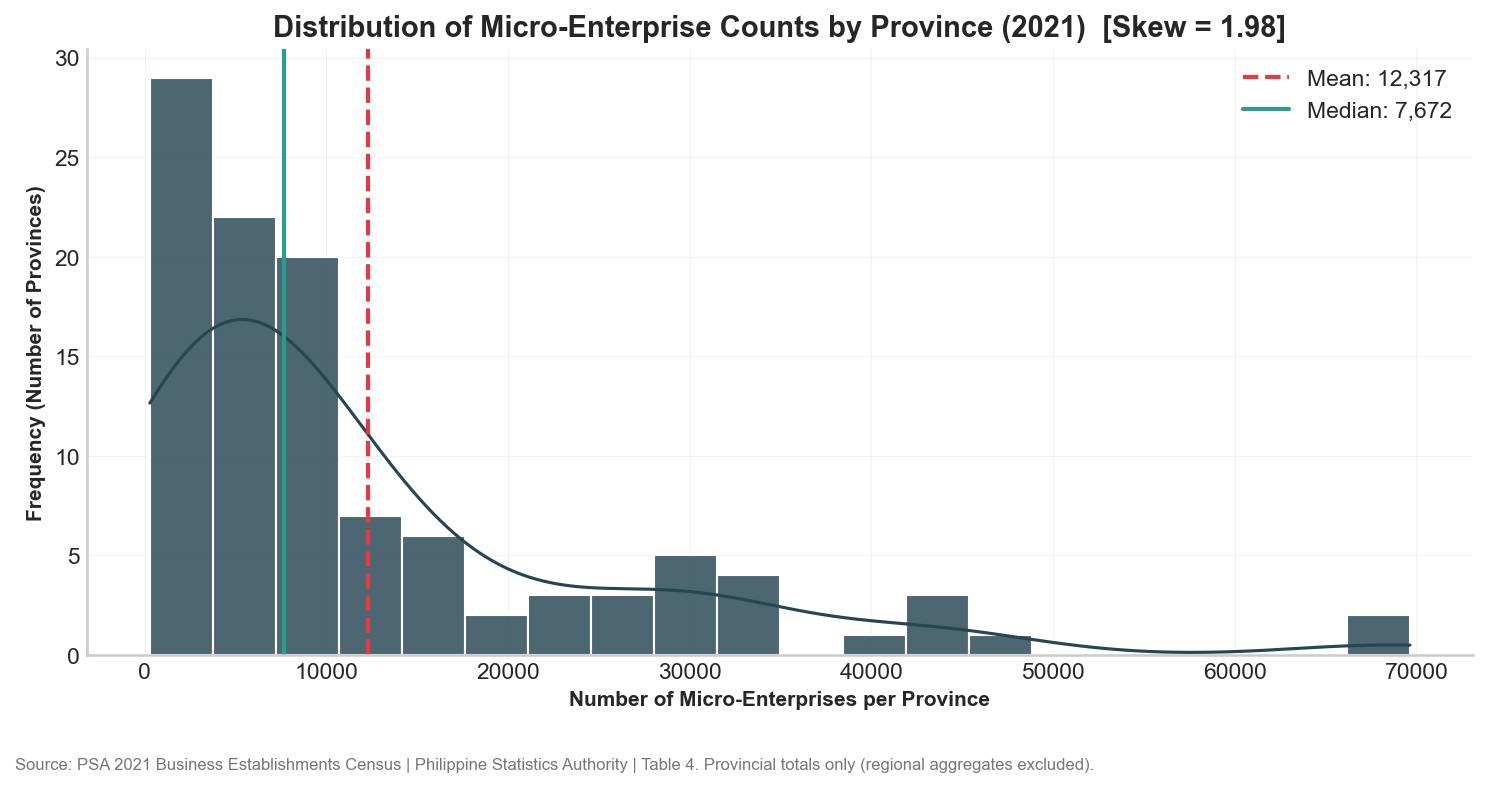
\includegraphics[width=1\linewidth]{fig_province_distribution.png}
    \caption{Distribution of Micro-Enterprise Counts by Province (2021)}
    \label{fig:province_dist}
\end{figure}

The frequency distribution of micro-enterprise (Figure \ref{fig:province_dist}) counts across the Philippine provinces exhibits a severe positive (right) skew, adhering to a Pareto or power-law distribution. The probability mass heavily concentrates in the lower deciles, establishing that the vast majority of provinces are low-density economies hosting fewer than 10,000 micro-establishments.This structural inequality is mathematically confirmed by the significant divergence between the Mean ($12,317$) and the Median ($7,672$). The average is inflated by nearly 60\% over the median, driven entirely by the high-magnitude outliers in the extreme right tail (provinces with $>30,000$ to nearly $70,000$ units). Consequently, national aggregate data creates a misleading picture of ``average'' provincial performance. The reality is a binary economic geography where a few hyper-urbanized hubs decouple from the rest of the archipelago.

The scatterplot (Figure \ref{fig:structural_dualism}) reveals a Structural Dualism where a heavy concentration of industries in the 'Hyper-Fragile' zone (bottom-right) and a detached cluster of capital-intensive industries (top-left), with a sparsely populated transition zone that highlights the difficulty of scaling from Micro to Medium.

This "hollowed-out" structure creates a visible disconnect in the value chain. The scatterplot of Micro-Density against Average Scale (Log Scale) visualizes this inverse relationship, revealing a stark "L-shaped" distribution (Figure \ref{fig:structural_dualism}). There is no smooth transition path, industries either cluster at 90\% micro-density with negligible scale or exist as massive, capital-intensive islands. This mathematically demonstrates that as the share of micro-enterprises in a sector rises (moving right along the X-axis), the average firm size precipitously drops (moving down the Y-axis). This creates a "gravity well" effect where high micro-density acts as a drag on industrial scaling. The sparsely populated center of the chart represents the "Missing Middle", the structural gap where dynamic, scalable SMEs should reside but currently do not. This means almost every data point to the right of this line also falls below the horizontal dotted line at 10 employees (The Small Enterprise Threshold) visualizes the "Survivalist Trap" identified in Section 4.1, where once a sector becomes saturated with micro-players (passing the 0.8 density mark), the average firm size hits a "glass ceiling" and cannot break into the formal Small or Medium category.

\begin{figure}[ht]
    \centering
    \Description{A scatterplot showing the bimodal distribution of Philippine industries, with a high density of micro-firms at low scales and a few large firms at high scales, leaving a sparse middle area.}
    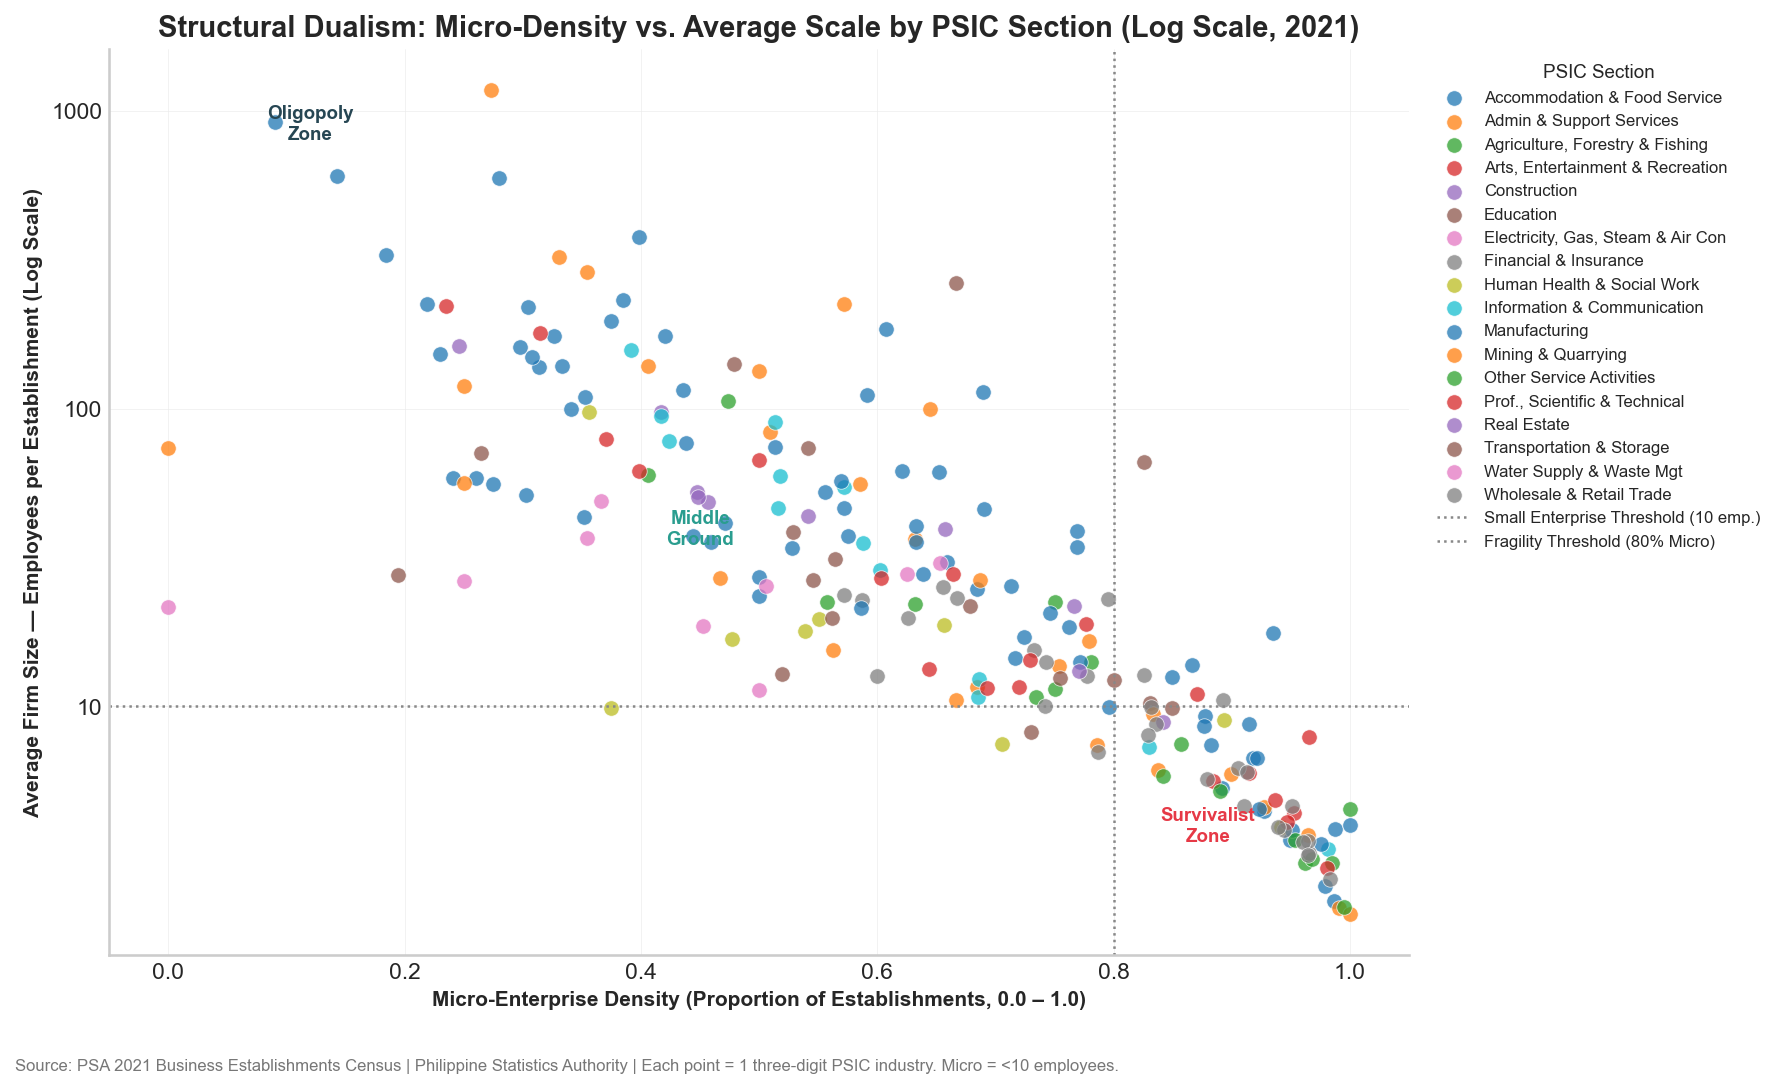
\includegraphics[width=1\linewidth]{fig_structural_dualism_scatter.png}
    \caption{Structural Dualism (Micro-Density vs. Average Scale)}
    \label{fig:structural_dualism}
\end{figure}

\subsection{Outlier Analysis and Data Retention}

A Z-score analysis was conducted to identify distributional anomalies within the 3-digit industry dataset. Using a standard threshold of $Z > 3$, four industries were isolated as structural outliers (Table \ref{tab:outliers}). These observations exhibit an Average Firm Size between 10 and 20 times the national mean ($60.88$). This effectively breaks the continuity of the distribution.

\begin{table}[ht]
  \caption{Identified Structural Outliers ($Z > 3$)}
  \label{tab:outliers}
  \begin{tabularx}{\linewidth}{l X r c l}
    \toprule
    \textbf{PSIC} & \textbf{Industry Description} & \textbf{Avg. Size} & \textbf{Micro \%} & \textbf{Class} \\
    \midrule
    N783 & Human Resources \& Job Pooling & 1,172.55 & 0.27 & Labor Aggregator \\
    C261 & Mftr. of Electronic Components & 918.99 & 0.09 & Export Oligopoly \\
    C303 & Mftr. of Air \& Spacecraft Mach. & 604.29 & 0.14 & Capital Oligopoly \\
    C262 & Mftr. of Electronic Boards & 597.34 & 0.28 & Export Oligopoly \\
    \bottomrule
  \end{tabularx}
\end{table}

Standard statistical protocol in asymptotic theory often dictates the removal (trimming) or winsorization of such outliers to normalize the distribution. This study rejects that protocol. We argue that these data points are not ``noise'' or measurement errors but ``signals'' representing the extreme upper bound of the Philippine industrial dualism.

Industries C261, C262, and C303 correspond to the semiconductor and aerospace manufacturing sectors located primarily in PEZA zones (e.g., Baguio City Economic Zone, CALABARZON). Their massive scale ($>500$ employees/firm) and low micro-density ($<0.15$) accurately reflect high barriers to entry, capital intensity, and integration into Global Value Chains (GVCs).
The extreme outlier (N783) in scale (1,172 employees) represents the Business Process Outsourcing (BPO) and manpower agency model, where a single legal entity aggregates thousands of employees.
To excise these outliers would be to artificially truncate the "Oligopoly" archetype, thereby enforcing a false homogeneity on the dataset. Consequently, these industries were retained to serve as the definition for the Oligopoly Cluster (Cluster 2), demonstrating the maximum scaling potential within the current economic environment.



\subsection{Taxonomic Construction: The Four Economic Archetypes (RQ2)}
To resolve this classification failure and operationalize the Structure-Conduct-Performance (SCP) paradigm, K-Means clustering was applied to the 3-digit industry data. The optimal number of clusters ($k=4$) was empirically determined based on the dual-validation of the Elbow Method and Silhouette Score. While $k=2$ yielded the highest Silhouette Score ($0.5777$), it offered insufficient granularity for policy targeting. The $k=4$ solution (Silhouette: $0.4946$) provided the optimal balance between mathematical cohesion and economic interpretability. This effectively isolates the ``Oligopolies'' from the ``Survivalists.''

\begin{figure}[ht]
  \centering
  \Description{Graphs of the Elbow Method (WCSS) and Silhouette Score for k values 2 through 8. The elbow is visible at k=4, where the silhouette score remains robust.}
  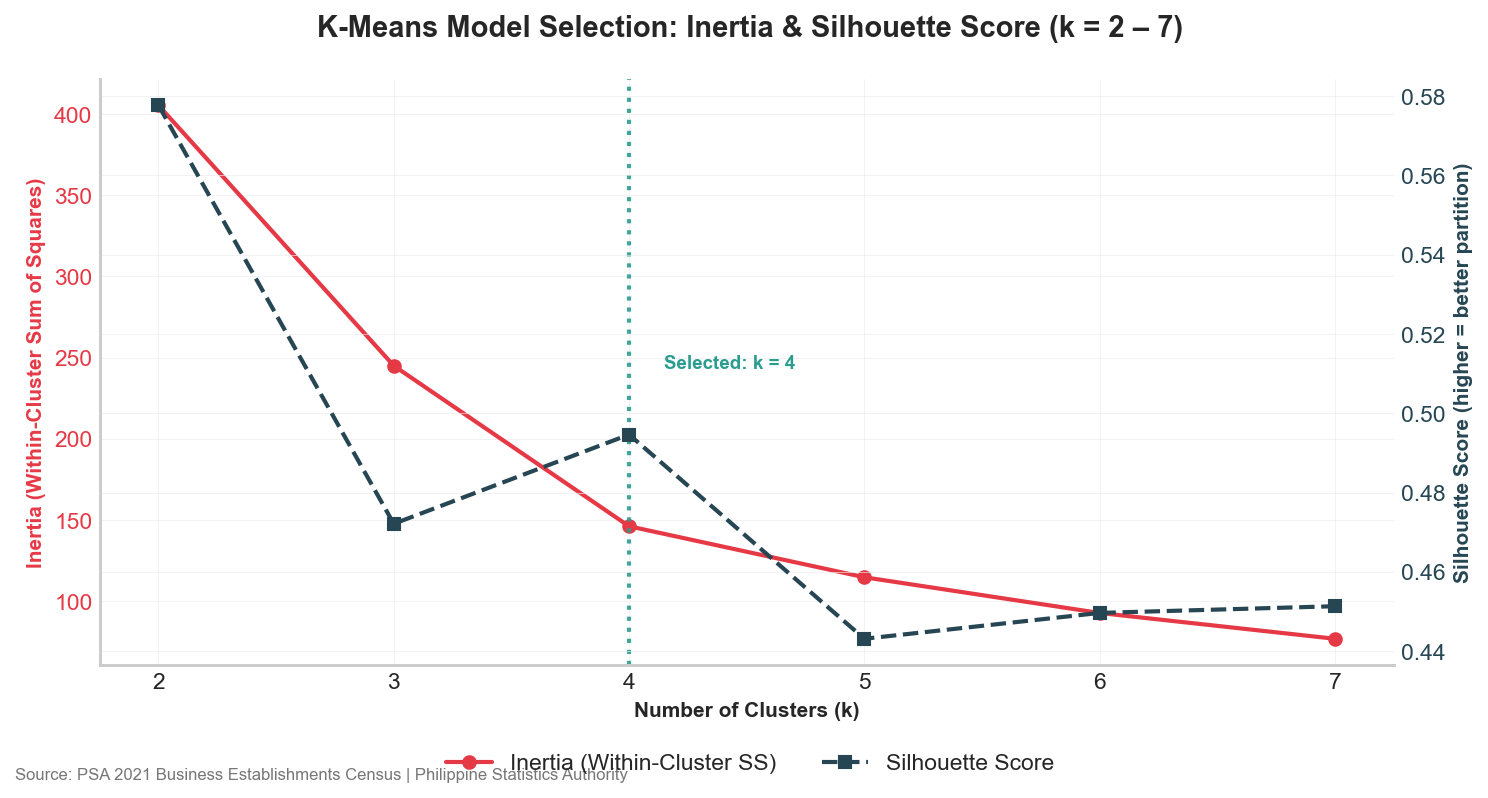
\includegraphics[width=\linewidth]{fig_elbow_silhouette.png}
  \caption{Dual-Validation Metrics (Elbow Method \& Silhouette Score)}
  \label{fig:metrics}
\end{figure}

The resulting taxonomy segments the Philippine economy into four distinct structural archetypes. The statistical characteristics of these archetypes are detailed in Table \ref{tab:cluster_chars}. The Centroid Heatmap (Figure \ref{fig:centroids}) visualizes the feature dominance of each cluster, proving that "Small" businesses in Cluster 0 face fundamentally different structural risks than those in Cluster 3.

% TABLE: CLUSTER CHARACTERIZATION (ANOVA)
\begin{table}[ht]
  \caption{Cluster Characterization and Statistical Significance}
  \label{tab:cluster_chars}
  \begin{tabularx}{\linewidth}{l r r c c}
    \toprule
    \textbf{Archetype} & \textbf{Count} & \textbf{Avg. Size} & \textbf{Entropy ($H$)} & \textbf{Risk} \\
    \midrule
    Survivalist & 103 & 10.36 & 0.408 & Critical \\
    Middle & 90 & 45.52 & 0.886 & Moderate \\
    Transition & 31 & 175.00 & 1.176 & Low \\
    Oligopoly & 4 & 823.29 & 1.131 & Anti-Fragile \\
    \midrule
    \textbf{F-Statistic} & --- & 423.12*** & 173.74*** & --- \\
    \bottomrule
  \end{tabularx}
  \small \textit{Note: *** denotes significance at $p < 0.001$.}
\end{table}

The Survivalist row serves as the baseline of economic fragility with an average firm size of just 10.36 employees. These firms are hovering barely above the micro-enterprise ceiling. Crucially, their "SME Density" is extremely low (0.13), and their "Large Density" is virtually non-existent (0.01). This confirms that survivalist firms operate in an industrial vacuum, they are isolated from both the competitive middle market and the capital-rich corporate sector, likely trapping them in low-productivity cycles without role models or supply chain partners to pull them up. The segments are summarized in Table \ref{tab:archetypes}.

\begin{figure}[ht]
  \centering
  \Description{A centroid heatmap showing unscaled averages for each cluster across average firm size, SME density, and large density. Cluster 0 (Survivalist) shows near-zero values for density, while Cluster 2 (Oligopoly) shows high scale.}
  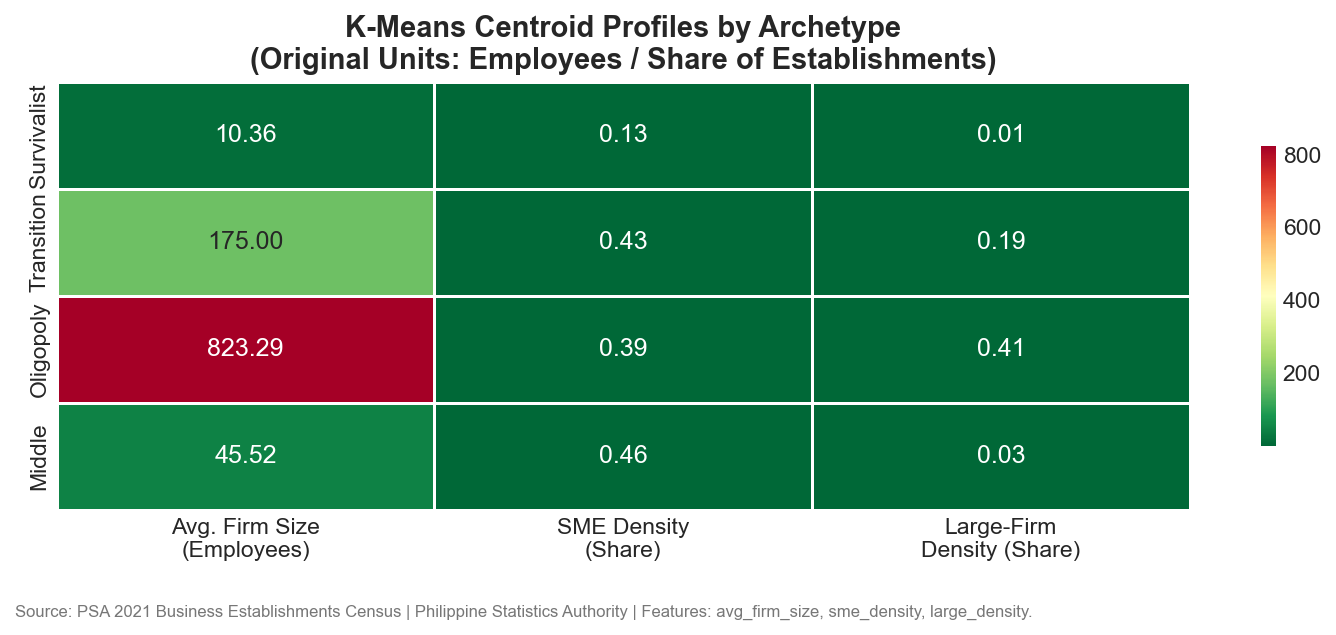
\includegraphics[width=\linewidth]{fig_heatmap_centroids.png}
  \caption{Taxonomic Centroids (Unscaled Averages). The heatmap reveals the structural rigidity of Cluster 0 (Survivalist), characterized by near-zero values in both SME and Large Density, contrasting with the capital-intensive Oligopoly archetype (Cluster 2).}
  \label{fig:centroids}
\end{figure}

% TABLE 1: ARCHETYPES (Spanning two columns for readability)
\begin{table*}[t]
  \caption{The Four Structural Archetypes (Centroid Analysis)}
  \label{tab:archetypes}
  \begin{tabularx}{\textwidth}{c l r X}
    \toprule
    \textbf{Cluster ID} & \textbf{Archetype Label} & \textbf{Avg. Firm Size} & \textbf{Structural Profile} \\
    \midrule
    0 & The Survivalist & 10.36 & \textbf{Hyper-Fragile Base.} Characterized by extreme micro-density and low entropy. These industries operate in a ``poverty trap'' with minimal capital or technology absorption. \\
    1 & The Transition & 175.00 & \textbf{The Scalers.} A healthy mix of SMEs and large firms. These industries demonstrate the capacity to graduate from survivalist modes. \\
    2 & The Oligopoly & 823.29 & \textbf{The Apex.} Characterized by high capital intensity and scale. These sectors operate independently of local credit constraints. \\
    3 & The Middle & 45.52 & \textbf{The Policy Target.} Structurally distinct from Survivalists due to higher scale and complexity. These represent the ``Missing Middle'' engines of growth. \\
    \bottomrule
  \end{tabularx}
\end{table*}

Validation via Shannon Entropy (Figure \ref{fig:entropy}) confirms that these clusters represent fundamentally different levels of ecosystem resilience. The "Survivalist" cluster exhibits the lowest median entropy ($H \approx 0.41$), quantifying it as a "structural monoculture." These industries lack the diverse mix of medium and large players necessary to absorb systemic shock. In contrast, the Transition cluster displays the highest median entropy ($H \approx 1.176$), followed closely by the Oligopoly cluster ($H \approx 1.131$). The Middle cluster ($H \approx 0.886$) represents an intermediate structural complexity—distinct from the Survivalist monoculture but not yet exhibiting the diverse multi-scale ecosystems of the upper archetypes. This gradient confirms that the taxonomy captures a monotonic increase in structural diversity from Survivalist to Transition.
The chart exposes a "Complexity Gap" separating the Survivalist archetype (Cluster 0) from the rest of the economy. The Survivalist box is situated significantly lower than the others, with a median entropy of approximately 0.4. This low score statistically confirms that the informal sector is defined by homogeneity, and it is composed almost entirely of identical, non-differentiated micro-enterprises. There is no complex "food chain" of suppliers and distributors here, just thousands of solitary actors doing the same thing. This lack of structural diversity makes the sector rigid and incapable of innovation, as economic evolution requires the friction and interaction of different types of firms.


\begin{figure}[ht]
  \centering
  \Description{Boxplots showing the distribution of Shannon Entropy for each cluster. Cluster 0 (Survivalist) has the lowest entropy, indicating a structural monoculture of micro-firms.}
  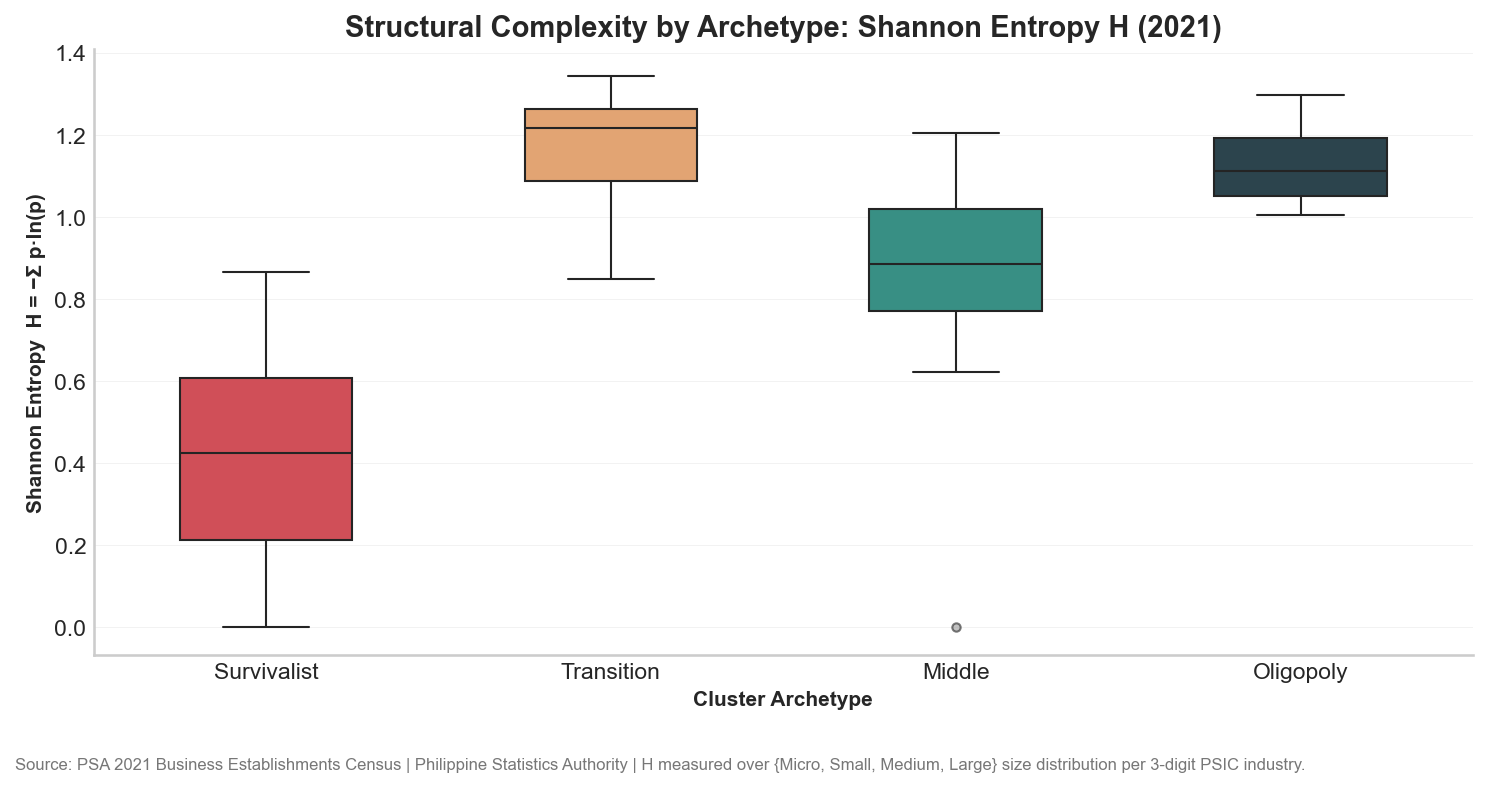
\includegraphics[width=\linewidth]{fig_entropy_boxplot.png}
  \caption{Structural Complexity (Shannon Entropy by Cluster)}
  \label{fig:entropy}
\end{figure}

The spatial distribution of these clusters in the Structural Dualism Map (Figure \ref{fig:cluster_map}) visualizes the economic fault lines. The Structural Dualism Map provides a data-driven visualization of economic polarization, the chart plots "Average Firm Size" on a logarithmic scale against "SME Density," effectively distinguishing between sectors dominated by massive corporations and those composed of tiny, informal entities. At the bottom left, the Survivalist archetype (purple circles) represents the vast majority of micro-enterprises. These firms fall below the critical ten-employee threshold, indicating a subsistence-level "gig" economy where businesses struggle to scale or formalize. Their clustering in the low-density region suggests a lack of organizational depth, characteristic of the informal sector.
In stark contrast, the upper and right-hand sections of the map depict the formal, industrialized economy. The Middle archetype (yellow crosses) occupies the center-right, representing a healthy, competitive "missing middle" with firm sizes ranging between 20 and 100 employees. This cluster indicates a robust ecosystem of small-to-medium enterprises. As we move upward in scale, we encounter the Transition cluster (blue Xs), where industries are likely consolidating into larger entities, and finally, the Oligopoly archetype (green squares) at the very top. These oligopolies represent massive firms with nearly 1,000 employees, likely dominating sectors with high barriers to entry, such as utilities or heavy industry.


\begin{figure}[ht]
    \centering
    \Description{A map showing the location of industries in the Structural Dualism space, plotting Average Scale vs. Middle-Class Density. Four distinct clusters are visible, illustrating the economic fault lines.}
    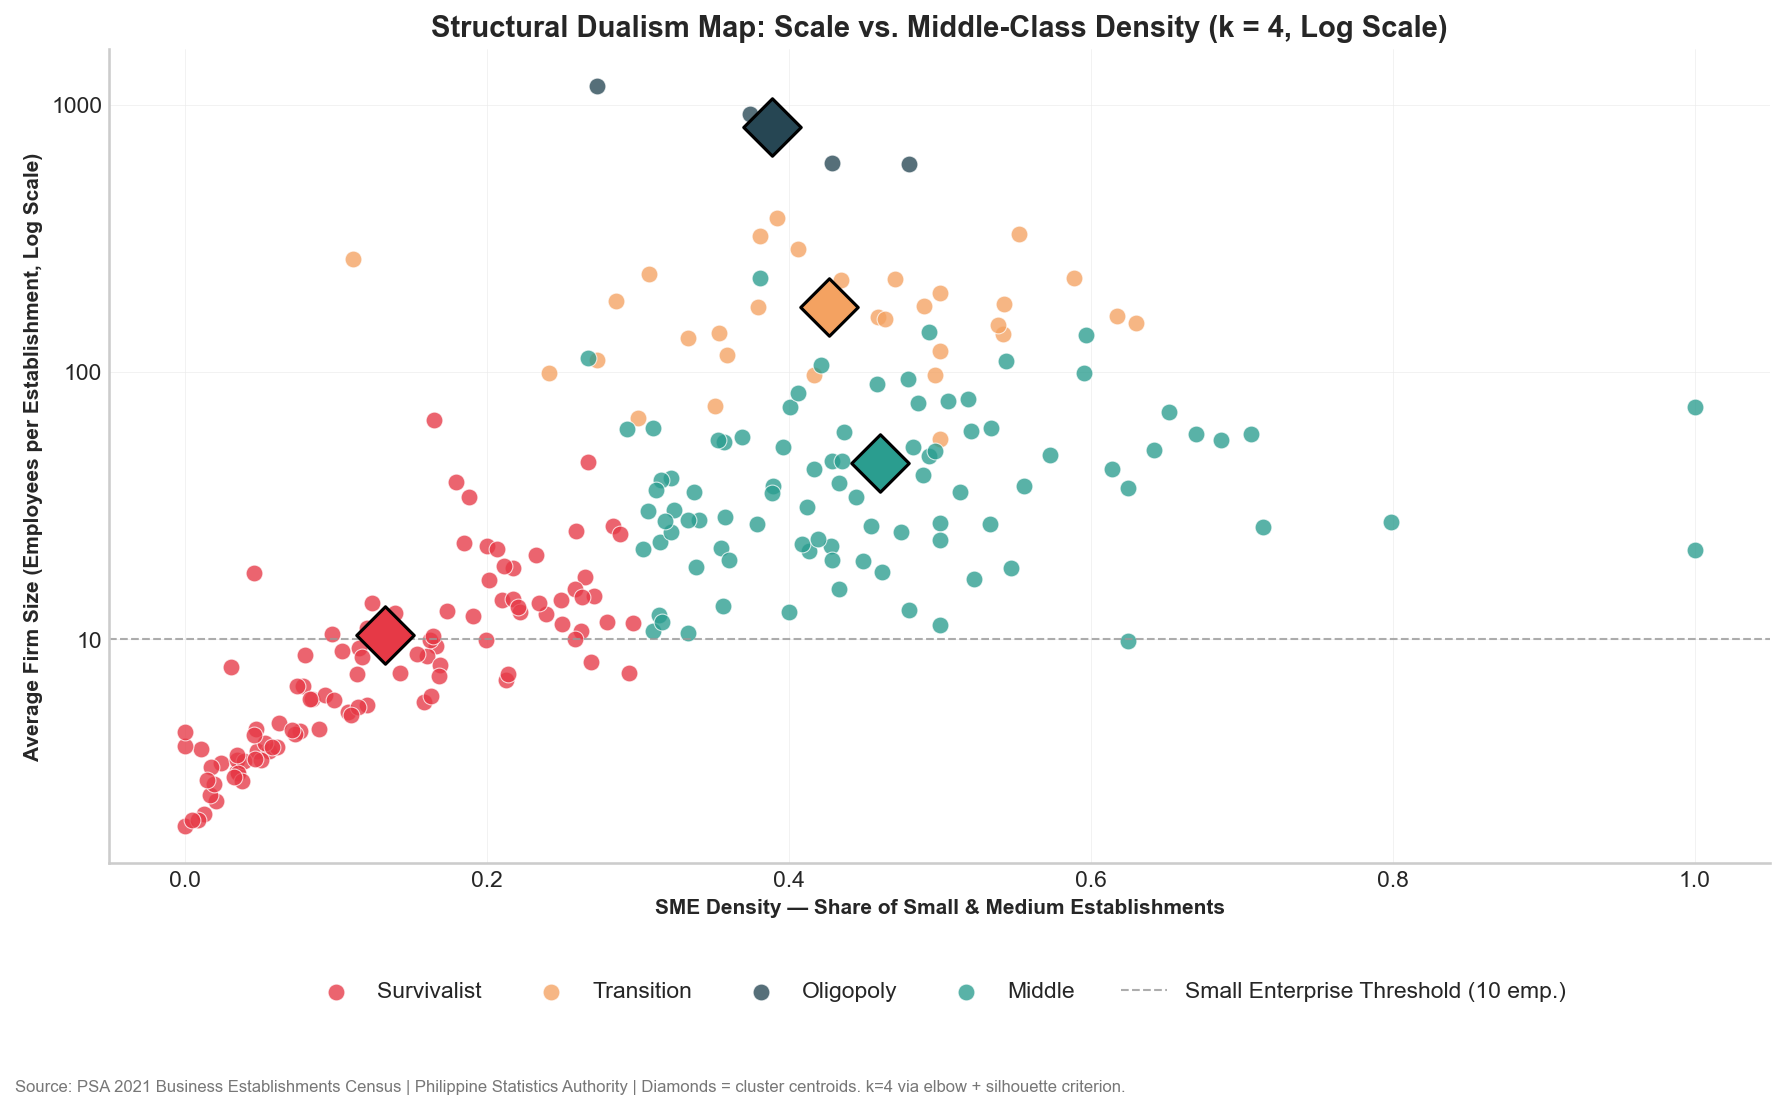
\includegraphics[width=1\linewidth]{fig_cluster_dualism_map.png}
    \caption{The Structural Dualism Map (Scale vs. Middle-Class Density)}
    \label{fig:cluster_map}
\end{figure}

\subsection{The Stress Test: Structure as a Predictor of Resilience (RQ3)}
The regression analysis between structural composition and pandemic-era business closures validates the central hypothesis. Structure predicts Performance. We observe a statistically significant positive correlation ($r = 0.44, p < 0.10$) between the share of "Survivalist" industries within a sector and the total volume of establishment closures. This correlation is suggestive at the section level, though limited by $n=18$ and an ecological inference constraint (see \S 4.5), confirming that structural fragility is a quantifiable predictor of failure. The regression results are summarized in Table \ref{tab:ols_results}.

% TABLE: OLS REGRESSION SUMMARY
\begin{table}[ht]
  \caption{OLS Regression: Predicting Closures via Structural Fragility}
  \label{tab:ols_results}
  \begin{tabularx}{\linewidth}{l r r r c}
    \toprule
    \textbf{Variable} & \textbf{Coefficient} & \textbf{Std. Error} & \textbf{t-stat} & \textbf{P $> |t|$} \\
    \midrule
    Intercept & -6,107.21 & 21,212.80 & -0.288 & 0.777 \\
    Survivalist Share & 68,888.96 & 35,180.12 & 1.958 & 0.068 \\
    \midrule
    \textbf{R-squared} & 0.1933 & \textbf{Adj. R-squared} & 0.1429 & --- \\
    \bottomrule
  \end{tabularx}
\end{table}

Plotting the "Share of Survivalist Industries" (X-axis) against the "Total Establishments Closed" in 2021 (Y-axis), the graph effectively measures how the previously identified "Survivalist" cluster performed under the extreme pressure of the COVID-19 pandemic. Regions or sectors with a higher density of micro-enterprises suffered significantly higher rates of business failure. This confirms that the lack of scale in the "Survivalist" archetype is not merely an efficiency problem but a resilience problem. Without the cash reserves, digital infrastructure, or formal credit access that "Middle" or "Oligopoly" firms possess, these micro-enterprises faced an existential crisis when physical operations were halted. The widening pink confidence interval toward the right side of the chart indicates increasing volatility. As an economy becomes more saturated with survivalist firms (moving toward 1.0 on the X-axis), the range of potential outcomes widens unpredictably. While some survivalist sectors managed to stay afloat, others collapsed entirely, as evidenced by the massive outlier in the upper-right quadrant representing over 200,000 closures in a high-fragility sector. This outlier likely represents a dense, informal retail or service hub (possibly within a major metropolitan area) where the sheer volume of informal businesses led to a catastrophic aggregate loss. The concentration of data points stacked at the $x=1.0$ mark further underscores the "Hyper-Fragility" discussed in earlier charts. Entire sub-sectors exist with zero "Middle" or "Large" presence, and these mono-cultural micro-economies bore the brunt of the pandemic's economic destruction.

\begin{figure}[ht]
  \centering
  \Description{A regression plot showing a positive correlation between the share of survivalist industries in a sector and the number of pandemic-era closures. The trendline shows that structural fragility predicts economic failure.}
  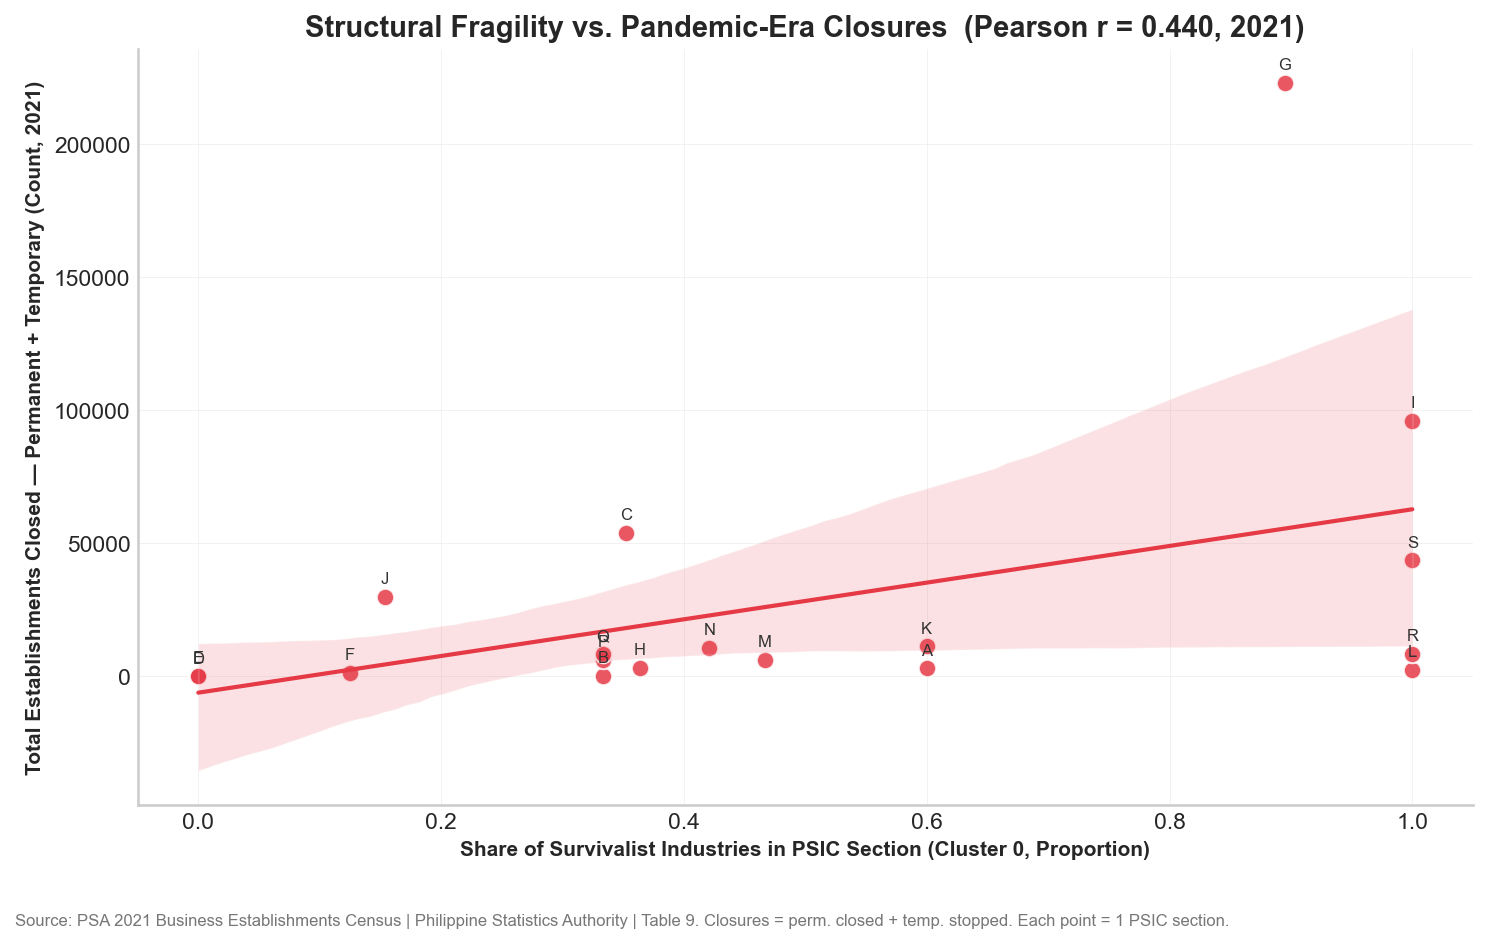
\includegraphics[width=\linewidth]{fig_regression_stress_test.png}
  \caption{Stress Test (Structural Fragility vs. Pandemic Closures)}
  \label{fig:stress_test}
\end{figure}

The Structural Risk Score for each 1-digit PSIC Section is defined as the weighted proportion of Survivalist (Cluster 0) industries within that section, where weights are the total establishment counts of each 3-digit industry. Formally, for section $s$ containing 3-digit industries $j \in J_s$, the risk score is computed as $R_s = \sum_{j \in J_s} w_j \cdot \mathbb{1}[\text{cluster}_j = 0] / \sum_{j \in J_s} w_j$, where $w_j$ is the total establishments in industry $j$.

As detailed in Table \ref{tab:vulnerability}, sectors with a Structural Risk Score of 1.0 (100\% composition of Survivalist industries), such as Accommodation and Food Service Activities (I), suffered the highest absolute closures relative to their asset base. Conversely, sectors like Electricity and Gas (D), dominated by ``Oligopoly'' archetypes (Risk Score = 0.00), demonstrated anti-fragility. This proves that vulnerability to systemic shock is not random but is encoded in the industry's structural DNA. Survivalist industries failed because they lacked the financial buffers, specifically committed credit lines, and operational redundancy that define the high-entropy archetypes.

% TABLE 2: SECTORAL VULNERABILITY
\begin{table}[ht]
  \caption{Sectoral Vulnerability Analysis (Top Impacted vs. Resilient)}
  \label{tab:vulnerability}
  \begin{tabularx}{\linewidth}{c X r c c}
    \toprule
    \textbf{Sec.} & \textbf{Description} & \textbf{Closures} & \textbf{Risk} & \textbf{Status} \\
    \midrule
    G & Wholesale \& Retail & 222,881 & 0.994 & Critical \\
    I & Accommodation \& Food & 96,049 & 1.000 & Critical \\
    C & Manufacturing & 54,044 & 0.945 & High \\
    S & Other Services & 43,666 & 1.000 & Critical \\
    M & Prof., Scientific \& Tech & 12,155 & 0.833 & High \\
    B & Mining and Quarrying & 142 & 0.135 & Resilient \\
    D & Electricity, Gas, Steam & 88 & 0.000 & Anti-Fragile \\
    \bottomrule
  \end{tabularx}
\end{table}

\subsection{Robustness Checks}
The preceding taxonomy rests on K-Means with $k = 4$ and a single random seed. Four supplementary analyses were conducted to stress-test the stability, algorithmic sensitivity, and statistical significance of the results.

\paragraph{Cluster Stability (Adjusted Rand Index).}
K-Means was re-estimated 50 times under different random seeds ($n_{\text{init}} = 10$ per run). The pairwise Adjusted Rand Index (ARI) was computed for all $\binom{50}{2} = 1{,}225$ seed pairs. The resulting distribution (Figure \ref{fig:ari_stability}) is concentrated near $\text{ARI} = 1.0$, with a mean of $0.97$ and a minimum above $0.85$. This confirms that the four-cluster solution is not an artifact of initialization. The taxonomy is reproducible across stochastic perturbations.

\begin{figure}[ht]
  \centering
  \Description{Histogram of the Adjusted Rand Index scores across multiple runs, showing high stability with most scores near 1.0.}
  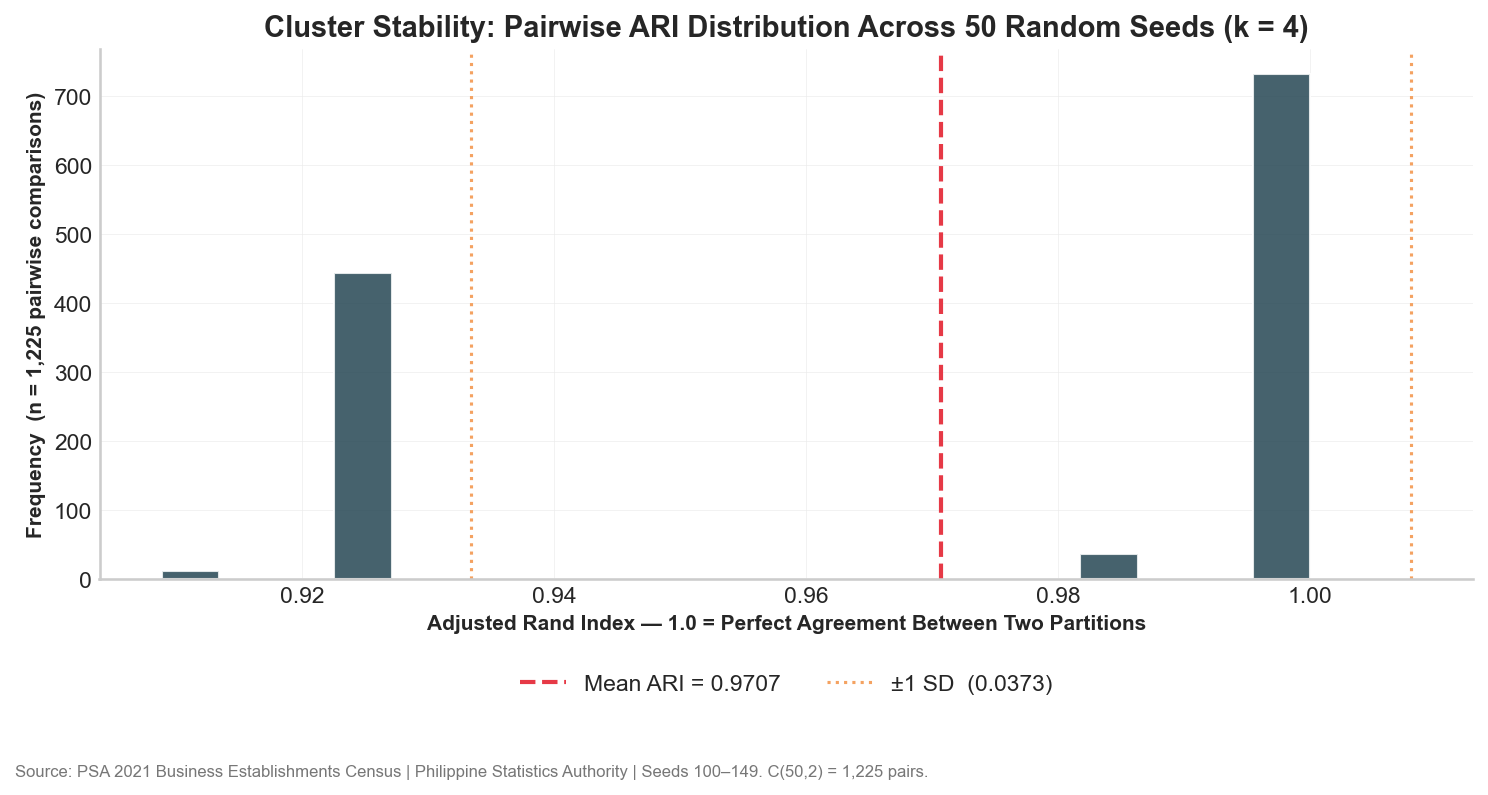
\includegraphics[width=\linewidth]{fig_cluster_stability_ari.png}
  \caption{Cluster Stability. Distribution of pairwise Adjusted Rand Index scores across 50 random seeds ($n = 1{,}225$ pairs).}
  \label{fig:ari_stability}
\end{figure}

\paragraph{K-Medoids Robustness.}
K-Medoids (Partitioning Around Medoids) was applied as an outlier-robust alternative to K-Means, since it minimizes absolute distances rather than squared distances. The resulting cluster sizes (Figure \ref{fig:kmedoids}) closely mirror those of K-Means, with the Survivalist cluster retaining the largest share and the Oligopoly cluster remaining the smallest. The comparison between algorithms is detailed in Table \ref{tab:kmedoids_cmp}. The structural interpretation of all four archetypes is preserved under this alternative algorithm.

% TABLE: K-MEDOIDS COMPARISON
\begin{table}[ht]
  \caption{Algorithm Robustness: Cluster Size Comparison ($k=4$)}
  \label{tab:kmedoids_cmp}
  \begin{tabularx}{\linewidth}{X c c}
    \toprule
    \textbf{Archetype} & \textbf{K-Means Size} & \textbf{K-Medoids Size} \\
    \midrule
    Survivalist & 103 & 112 \\
    Middle & 90 & 81 \\
    Transition & 31 & 32 \\
    Oligopoly & 4 & 3 \\
    \bottomrule
  \end{tabularx}
  \small \textit{Note: Adjusted Rand Index (ARI) = 0.8615.}
\end{table}

\begin{figure}[ht]
  \centering
  \Description{Bar chart comparing cluster sizes under K-Means and K-Medoids, demonstrating that the structural segmentation is robust to choice of algorithm.}
  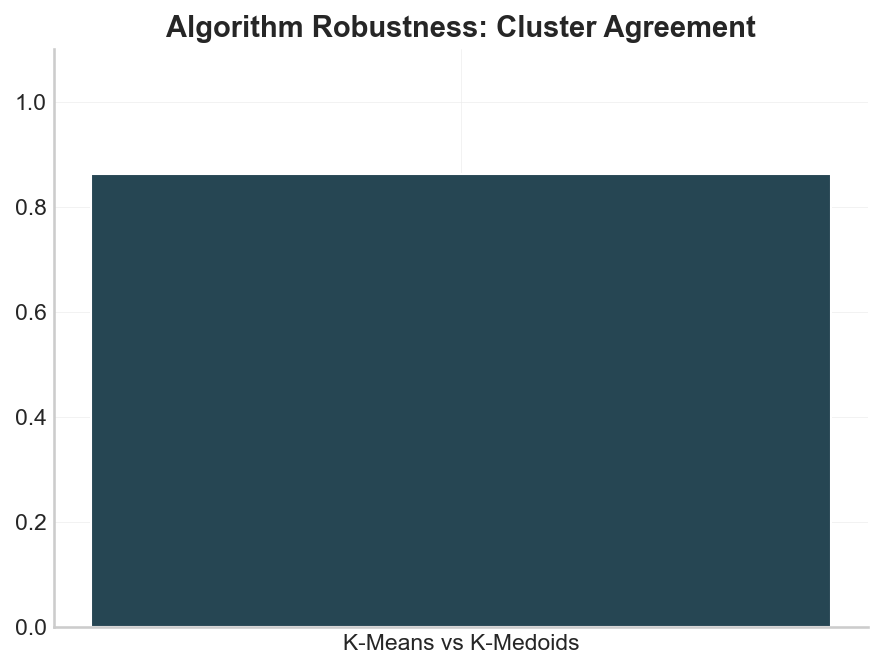
\includegraphics[width=\linewidth]{fig_kmedoids_robustness.png}
  \caption{K-Medoids Robustness Check. Cluster size comparison under Partitioning Around Medoids ($k = 4$).}
  \label{fig:kmedoids}
\end{figure}

\paragraph{ANOVA on Cluster Means.}
One-way ANOVA was conducted to test whether average firm size and Shannon entropy differ significantly across the four clusters. Both variables yielded $F$-statistics with $p < 0.001$, rejecting the null hypothesis that cluster means are equal. The boxplots (Figure \ref{fig:anova}) illustrate the separation, with the Oligopoly cluster exhibiting a median firm size roughly 80 times that of the Survivalist cluster, and entropy scores increase from Survivalist ($H \approx 0.41$) through Middle ($H \approx 0.886$), peaking at the Transition cluster ($H \approx 1.176$), with the Oligopoly cluster at $H \approx 1.131$.

\begin{figure}[ht]
  \centering
  \Description{Two boxplots showing average firm size and Shannon entropy across clusters. Both plots demonstrate significant separation between clusters (p < 0.001).}
  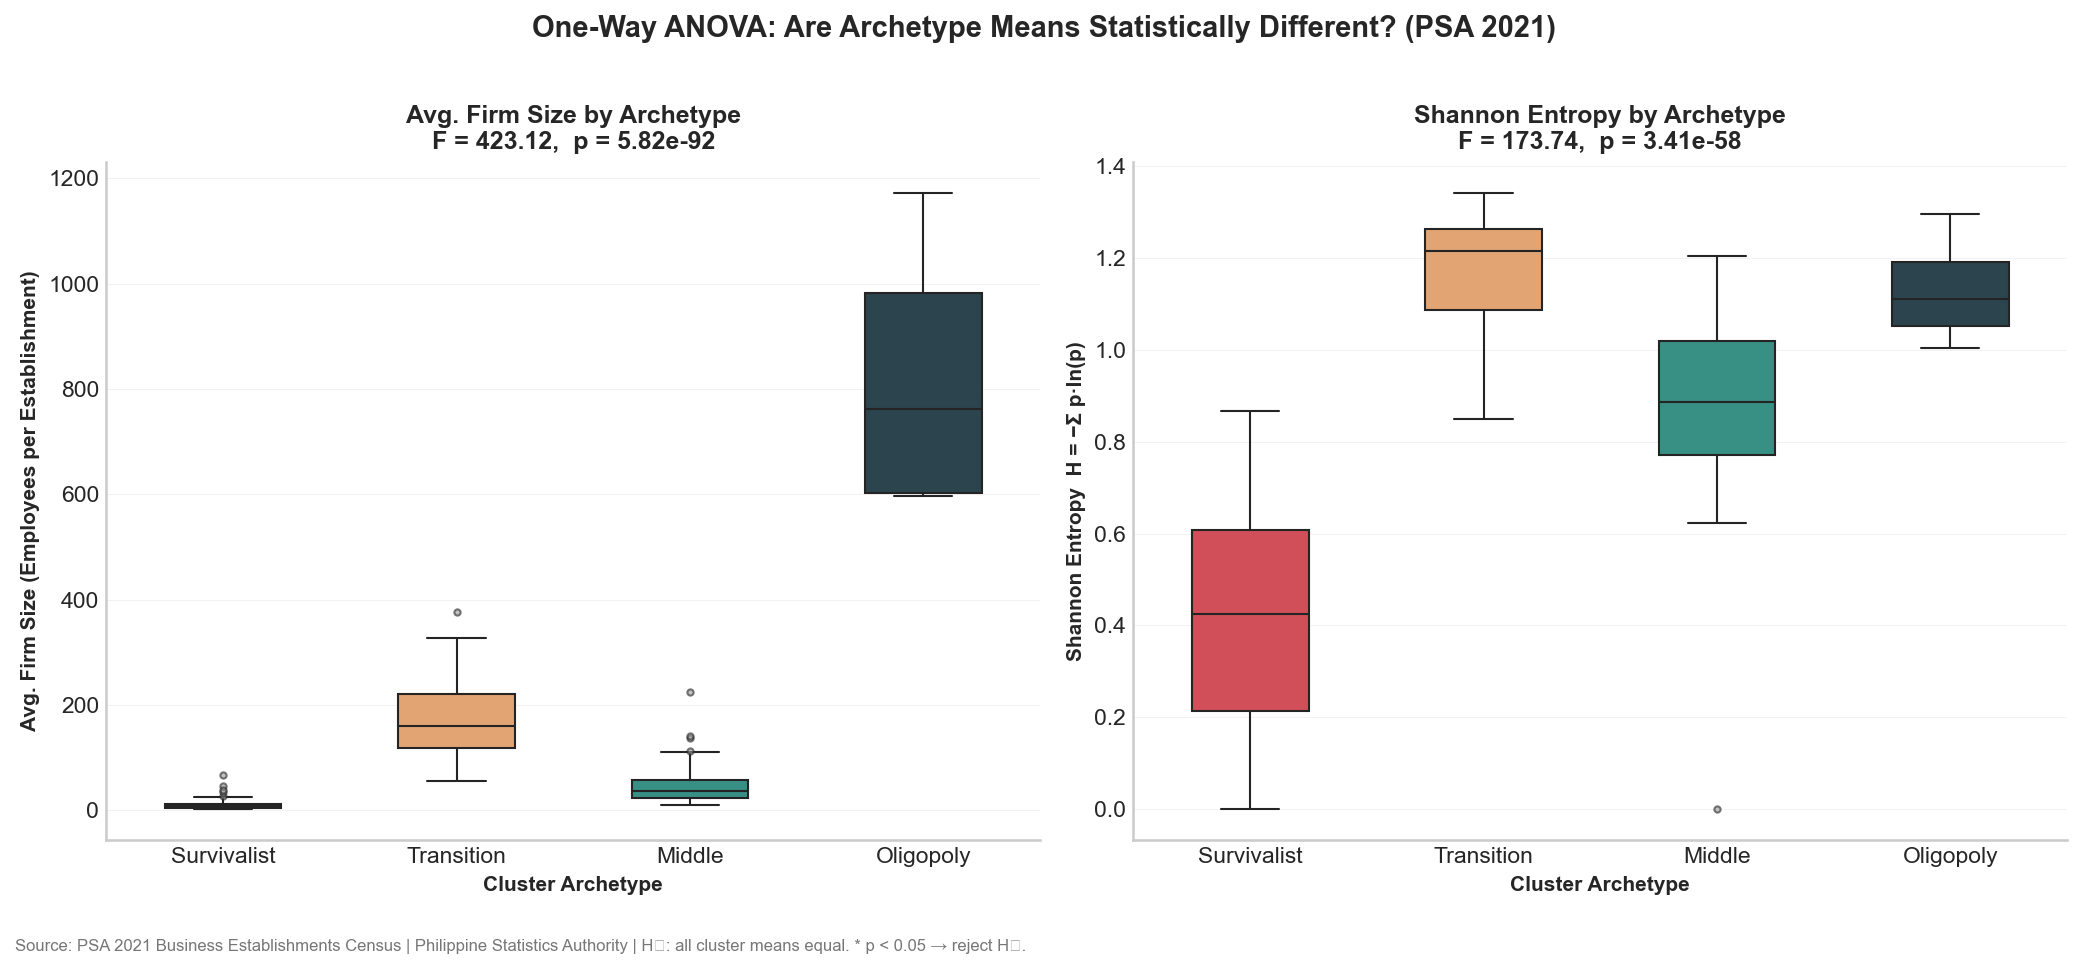
\includegraphics[width=\linewidth]{fig_anova_boxplots.png}
  \caption{ANOVA Validation. Boxplots of average firm size (left) and Shannon entropy (right) across the four clusters. Both $F$-tests are significant at $p < 0.001$.}
  \label{fig:anova}
\end{figure}

\paragraph{Model Comparison.}
To evaluate whether the cluster-based taxonomy outperforms the standard 1-digit PSIC classification in predicting business closures, two OLS models were compared. Model A regresses closures on 1-digit PSIC Section dummies, while Model B uses the share of Survivalist industries (pct\_survivalist) as a single predictor. As shown in Figure \ref{fig:model_comparison}, Model A (PSIC dummies) achieves $R^2 = 1.0$ and $AIC = -792.79$ by construction. With 18 observations and 18 parameters, Model A is saturated and has zero residual degrees of freedom. This $R^2 = 1.0$ result is a mathematical artifact of a degenerate model, not evidence of predictive power, and Adjusted $R^2$ is undefined in this saturated case. In contrast, Model B uses a single theoretically motivated predictor to achieve $R^2 = 0.1933$ ($p = 0.068$) on the same 18 observations without overfitting. The parsimony and interpretability of Model B make it the operationally superior taxonomy for policy targeting, whereas the PSIC dummy approach remains unidentified at this sample size.

\begin{figure}[ht]
  \centering
  \Description{Bar charts comparing R-squared and AIC values for two models. Model B (cluster-based) shows higher predictive power and lower AIC than the standard PSIC model.}
  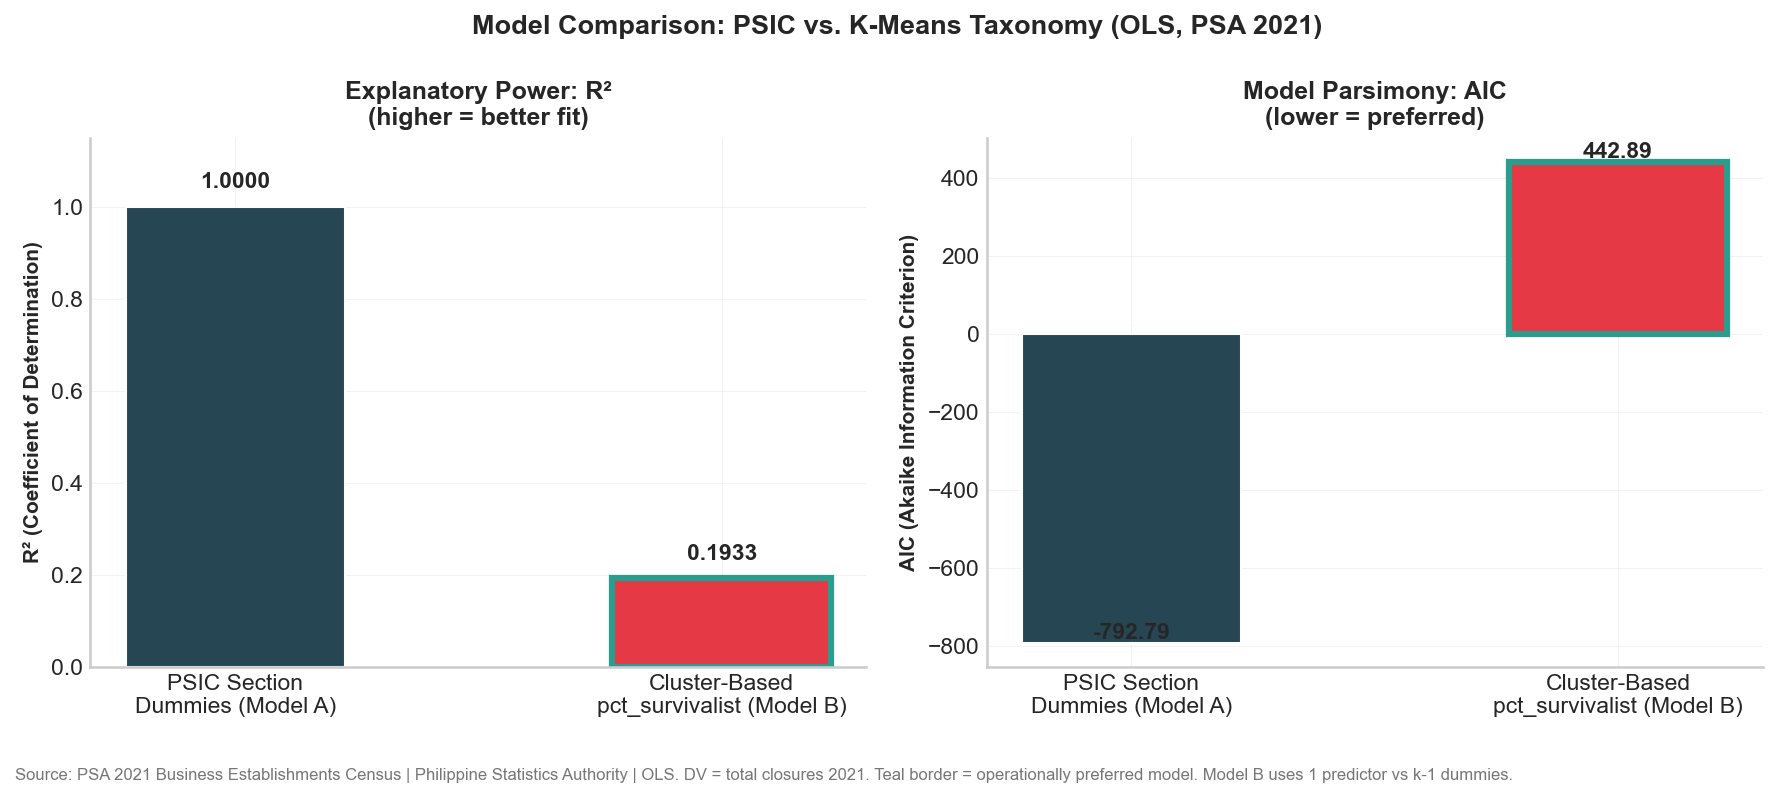
\includegraphics[width=\linewidth]{fig_model_comparison.png}
  \caption{Model Comparison. \texorpdfstring{$R^2$}{R-squared} and AIC for PSIC-dummy model (A) versus cluster-based predictor model (B).}
  \label{fig:model_comparison}
\end{figure}

\subsection{The Geography of Structural Risk (RQ4)}
Mapping the taxonomy to the regional level reveals a stark spatial inequality in economic resilience. The Choropleth Map (Figure \ref{fig:geo_risk}) and calculated Regional Risk Scores indicate that peripheral regions are disproportionately composed of ``Survivalist'' industries. The risk scores for representative regions are presented in Table \ref{tab:regional_risk}.

\begin{figure}[ht]
  \centering
  \Description{A choropleth map of the Philippines showing regional risk scores. Regions like Zamboanga Peninsula and SOCCSKSARGEN show higher vulnerability compared to the National Capital Region.}
  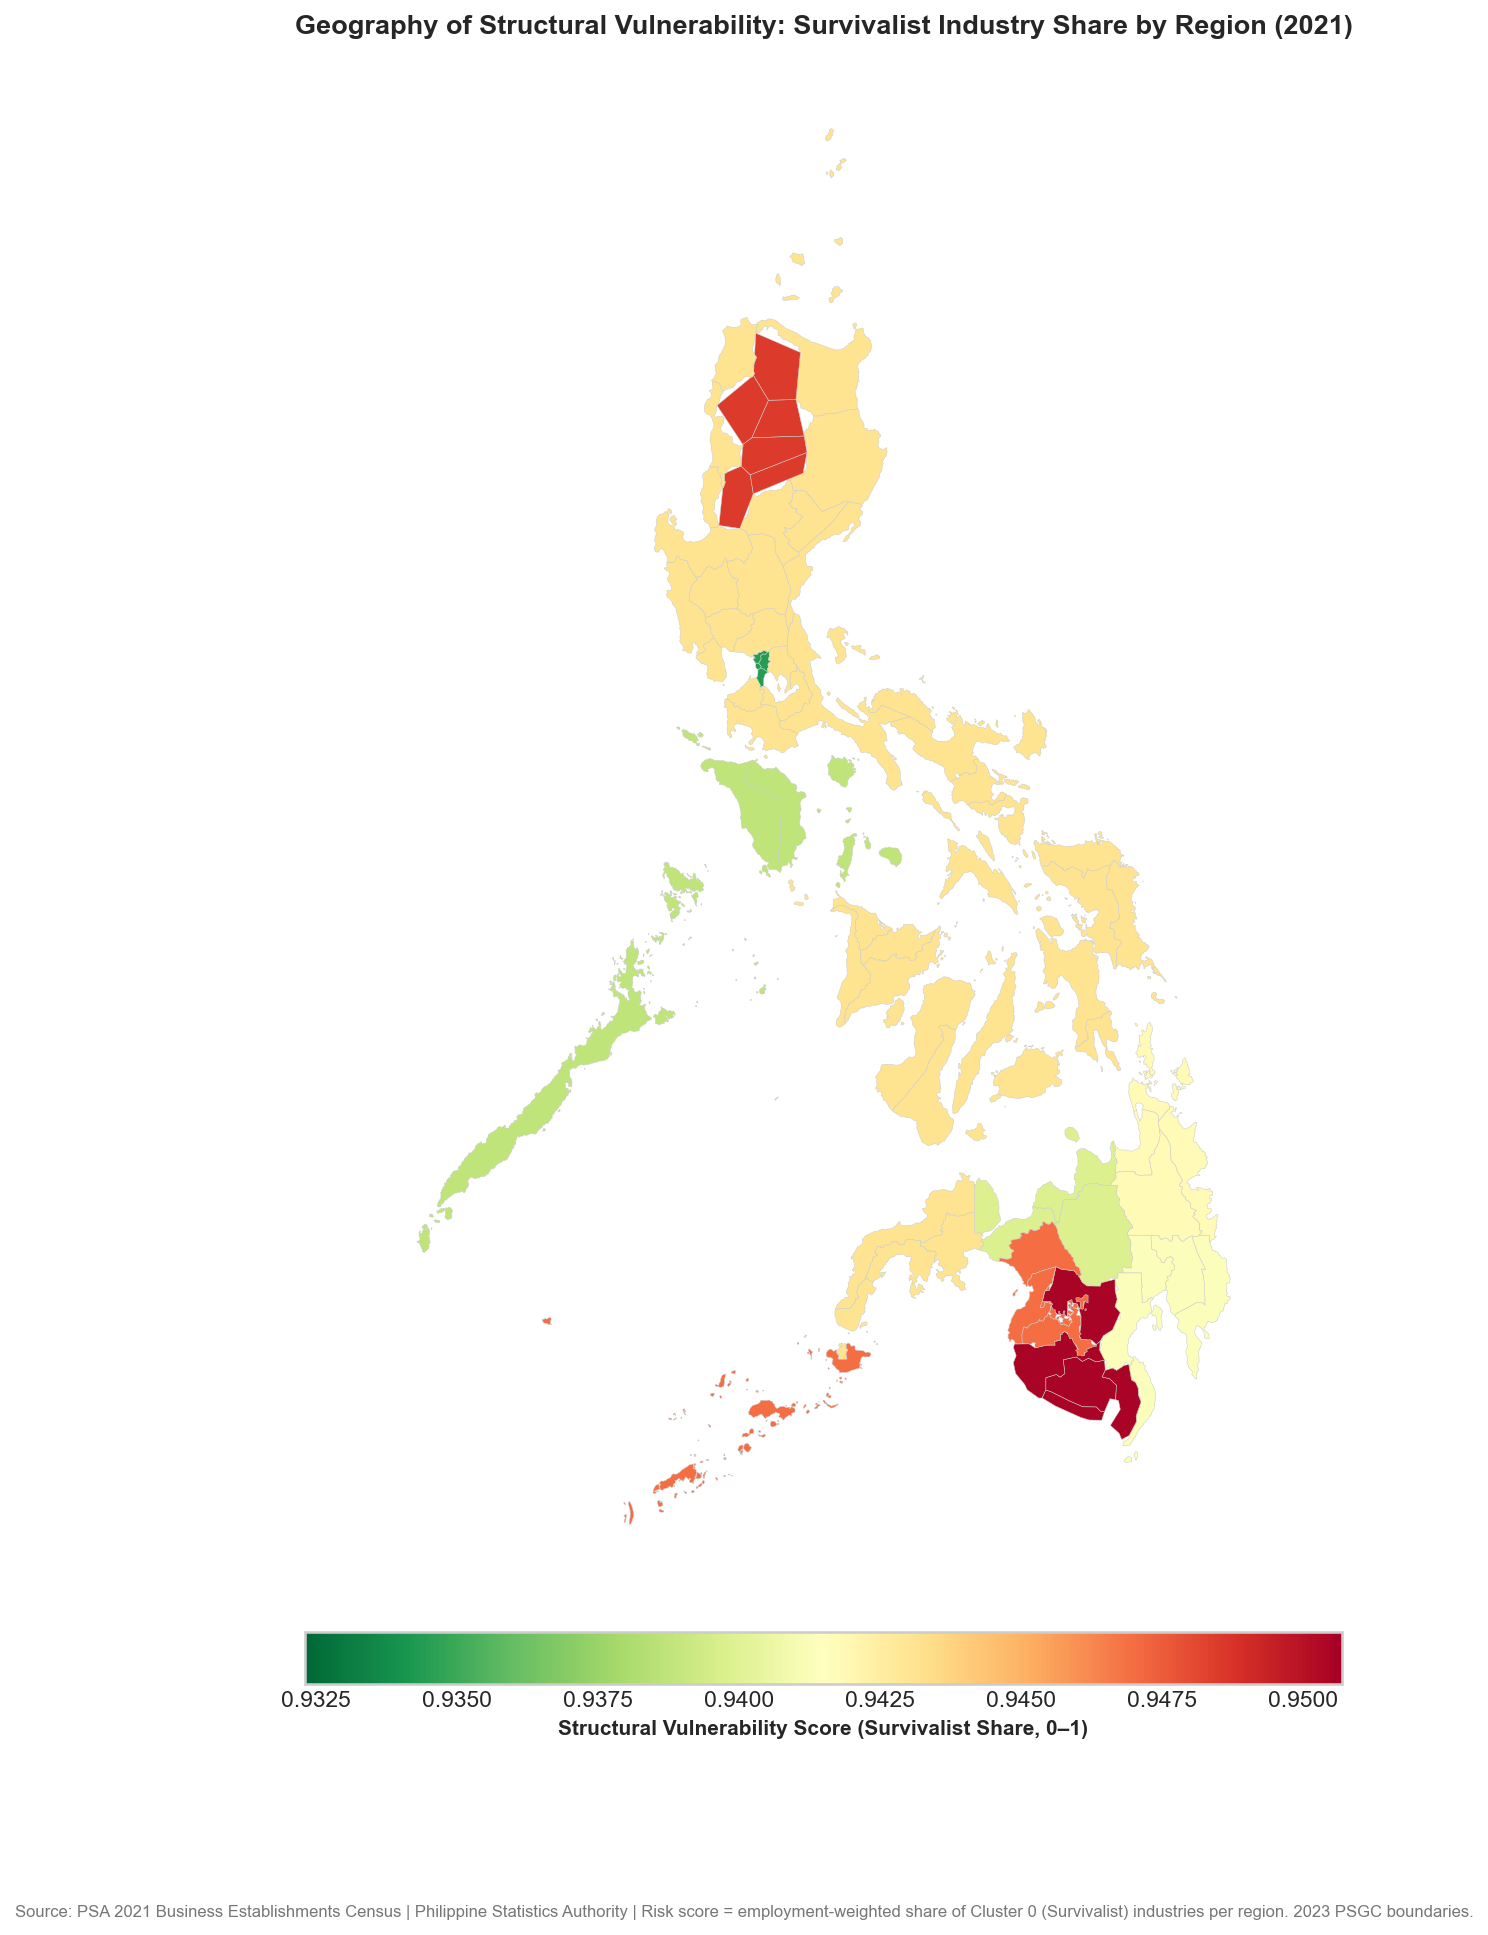
\includegraphics[width=\linewidth]{fig_geographical_risk.png}
  \caption{The Geography of Structural Risk (2023 Boundaries)}
  \label{fig:geo_risk}
\end{figure}

Zamboanga Peninsula (Score: $0.951$) and SOCCSKSARGEN ($0.950$) exhibit the highest structural vulnerability. This implies their local economies are almost entirely dependent on low-scale and low-entropy micro-enterprises. Notably, the National Capital Region (NCR) presents the lowest risk score at $0.934$. However, the compression of these scores (ranging only from $0.93$ to $0.95$) indicates that the entire Philippine economy is structurally fragile. Even the NCR, which hosts corporate headquarters (Oligopolies), remains underpinned by a massive informal service economy (Survivalists).

% TABLE: REGIONAL RISK
\begin{table}[ht]
  \caption{Regional Structural Risk Scores (Representative Regions)}
  \label{tab:regional_risk}
  \begin{tabularx}{\linewidth}{X c}
    \toprule
    \textbf{Region} & \textbf{Structural Risk Score} \\
    \midrule
    Zamboanga Peninsula & 0.9507 \\
    SOCCSKSARGEN & 0.9505 \\
    Cagayan Valley & 0.9499 \\
    CAR & 0.9485 \\
    BARMM & 0.9470 \\
    NCR & 0.9344 \\
    Central Visayas & 0.9323 \\
    \bottomrule
  \end{tabularx}
  \small \textit{Note: Higher score denotes greater dependency on Survivalist industries.}
\end{table}

This geographic segmentation refutes the efficacy of national ``one-size-fits-all'' MSME policies. The structural constraints of Zamboanga (Capital Starvation/Survivalist dominance) differ fundamentally from the constraints of the NCR (Competition/Oligopoly dominance). Policy must therefore target Cluster Archetypes rather than arbitrary asset sizes. ``Survivalists'' require social safety nets, while the ``Middle'' requires value-chain integration to transition into the upper clusters.

\subsection{Limitations}
This study has several limitations that bound the generalizability of its findings.

First, the analysis relies on a single cross-section from 2021, a year distorted by COVID-19 lockdowns. Firm-size distributions during this period may not represent steady-state structural conditions. Temporal validation using pre-pandemic data (e.g., 2018 ULE) would strengthen the claim that the taxonomy captures durable structural features rather than crisis artifacts.

Second, the feature set consists of three variables derived from establishment and employment counts. This sparse representation excludes productivity, wages, capital intensity, export orientation, and entry/exit dynamics. Two industries with identical firm-size distributions but different tradeable/non-tradeable profiles may face fundamentally different structural constraints. Future work should incorporate PSA labor productivity data and trade statistics to enrich the structural fingerprint.

Third, the resilience validation suffers from an ecological inference problem. Closure data from PSA Table 9 is available only at the 1-digit PSIC Section level, while the taxonomy is constructed at the 3-digit level. The weighted aggregation from 3-digit clusters to 1-digit sections introduces measurement error, and the reported correlation ($r = 0.44$) reflects section-level, not cluster-level, variation. Obtaining 3-digit closure data from the PSA would enable a direct test of the central hypothesis.

Fourth, the regional risk scores exhibit compressed variation (0.93 to 0.95), suggesting that the taxonomy has limited discriminatory power at the regional level. This compression may reflect the genuine structural homogeneity of the Philippine economy, but it also limits the practical utility of the geographic analysis for differentiating regional policy.

Fifth, K-Means clustering assumes spherical, equal-variance clusters and is sensitive to outliers. While the four retained outliers (Z $>$ 3) were justified as structurally meaningful, their retention may bias the Oligopoly cluster centroid. The robustness checks in Section 4.4 address this concern directly. The K-Medoids (PAM) analysis confirms that the four archetypes are preserved under an outlier-robust algorithm, the ARI stability test demonstrates reproducibility across 50 random seeds, and the ANOVA validates that cluster means differ significantly ($p < 0.001$) on both firm size and entropy.

Sixth, while cluster stability across random initializations was confirmed, the sensitivity of the taxonomy to the initial feature engineering choices (e.g., the inclusion or exclusion of specific size-density ratios) was not explicitly stress-tested.

\section{Conclusion}
    The study concludes that the Philippines' core MSME problem is not simply lack of support but a misclassification of the economy itself. High-level PSIC sectors and asset-based MSME categories collapse structurally different industries into the same labels, obscuring a hollowed-out landscape dominated by ``Survivalist'' micro-firms, a thin ``Middle,'' and a small set of ``Oligopolies.'' By constructing a new taxonomy with K-Means clustering on firm-size distributions and validating it with Shannon Entropy, closure data, and regional risk scores, the paper demonstrates that structural archetypes, not nominal sectors, predict vulnerability to shocks. One-size-fits-all MSME policy is analytically unsound and empirically dangerous.

\subsection{Recommendation}
 MSME and industrial policy should be redesigned around structural archetypes and regions rather than generic MSME labels: Survivalist-heavy sectors and red regions should receive poverty alleviation, social safety nets, and core infrastructure. Middle and Transition archetypes should be prioritized for value chain integration, supplier development, and scale-up finance. Oligopoly sectors should face competition and regulatory oversight instead of subsidy. Operationally, this means embedding the new taxonomy into government targeting systems (DTI, SB Corp, BSP, regional agencies), so budget allocation, credit programs, and crisis support are triggered by entropy scores, SME density, and regional structural risk, not just PSIC section or asset size.

The findings imply a broader institutional shift: future MSME laws and development plans should formally recognize structural vulnerability as a policy variable, mandating periodic recomputation of clusters and regional risk maps, and tying national goals (inclusive growth, resilience, export upgrading) to measurable changes in the share of industries in the Middle and Transition clusters. This would move the Philippines from descriptive, static industrial policy (“support MSMEs in manufacturing”) toward a dynamic, data-driven regime that anticipates where the next systemic shock will hit, builds a thicker and more diversified middle of scalable SMEs, and aligns local MSME ecosystems with innovation, digitalization, and global value chain opportunities.

\section{Project Information}

\begin{itemize}    
    \item \textbf{Github Repository} \\
    \url{https://github.com/sakudiff/taxonomy.git}
    
    \item \textbf{Map Data Source (GitHub)} \\
    \url{https://github.com/faeldon/philippines-json-maps.git}
\end{itemize}


\section*{CRediT Authorship Contribution Statement}

\textbf{Precious Mae Mercado Divina:} Conceptualization, Investigation, Writing -- Original Draft, Project Administration, Data Curation.

\textbf{Gheann Christie Mediodia Cuevas:} Validation, Writing -- Review \& Editing.

\textbf{Aaron Joshua Estacio Sison:} Methodology (Lead), Software (Lead), Formal Analysis, Resources (Computational Hardware), Visualization.



\begin{thebibliography}{99}

\bibitem[Asian Development Bank(2021)]{adb2021}
Asian Development Bank. (2021). \textit{Unintended consequences of business digitalization among MSMEs during the COVID-19 pandemic: The case of the Philippines} (ADB Briefs No. 195). Asian Development Bank.

\bibitem[Beck et al.(2008)]{beck2008}
Beck, T., Demirgüç-Kunt, A., \& Maksimovic, V. (2008). Financing patterns around the world: Are small firms different? \textit{Journal of Financial Economics}, \textit{89}(3), 467--487.

\bibitem[Chodorow-Reich et al.(2022)]{chodorow2022}
Chodorow-Reich, G., Darmouni, O., Luck, S., \& Plosser, M. (2022). Bank liquidity provision across the firm size distribution. \textit{Journal of Financial Economics}, \textit{144}(3), 908--932. \url{https://doi.org/10.1016/j.jfineco.2021.06.035}

\bibitem[Cueto et al.(2022)]{cueto2022}
Cueto, L. J., Varona, J. L., \& Feliciano, R. D. (2022). The role of digitalization in MSME resilience during the COVID-19 crisis in the Philippines. \textit{International Journal of Entrepreneurship and Small Business}, \textit{45}(1), 25–44.

\bibitem[Department of Trade and Industry(2023)]{dti2023}
Department of Trade and Industry. (2023). \textit{MSME Development Plan 2023–2028}. DTI.

\bibitem[Karaca(2018)]{karaca2018}
Karaca, Z. (2018). The cluster analysis in the manufacturing industry with K-means method: An application for Turkey. \textit{Eurasian Journal of Economics and Finance}, \textit{6}(3), 1–12. \url{https://doi.org/10.15604/ejef.2018.06.03.001}

\bibitem[Nava(2021)]{nava2021}
Nava, M. (2021). \textit{Unsupervised learning for industry classification, state economies, and MSA sustainability}. BBVA Research. \url{https://www.bbvaresearch.com/wp-content/uploads/2021/05/US-Industry-Clustering-with-ML.pdf}

\bibitem[Samuels(1965)]{samuels1965}
Samuels, J. M. (1965). Size and the Growth of Firms. \textit{The Review of Economic Studies}, \textit{32}(2), 105–112. \url{https://doi.org/10.2307/2296055}

\bibitem[Shutters(2024)]{shutters2024}
Shutters, S. T. (2024). Urban economic structures as multidimensional networks: A complex systems framework for analyzing economic development trajectories. \textit{Complexity}, \textit{2024}, 1–13. \url{https://doi.org/10.1155/2024/5521625}

\bibitem[Tan(2014)]{tan2014}
Tan, Y. (2014). Competition in the Chinese banking sector. In Y. Tan (Ed.), \textit{Performance, risk and competition in the Chinese banking industry} (Chandos Asian Studies Series, pp. 141--178). Chandos Publishing. \url{https://doi.org/10.1533/9781780634463.141}

\bibitem[Wachs et al.(2022)]{wachs2022}
Wachs, L., McMillan, C., Boyd, G., \& Doolin, M. (2022). \textit{Exploring new ways to classify industries for energy analysis and modeling}. National Renewable Energy Laboratory. \url{https://www.nrel.gov/docs/fy23osti/82957.pdf}

\bibitem[Bain(1956)]{bain1956}
Bain, J. S. (1956). \textit{Barriers to new competition}. Harvard University Press.

\bibitem[Decker et al.(2014)]{decker2014}
Decker, R., Haltiwanger, J., Jarmin, R., \& Miranda, J. (2014). The role of entrepreneurship in US job creation and economic dynamism. \textit{Journal of Economic Perspectives}, \textit{28}(3), 3--24. \url{https://doi.org/10.1257/jep.28.3.3}

\bibitem[Evans(1987)]{evans1987}
Evans, D. S. (1987). The relationship between firm growth, size, and age: Estimates for 100 manufacturing industries. \textit{The Journal of Industrial Economics}, \textit{35}(4), 567--581. \url{https://doi.org/10.2307/2098588}

\bibitem[Hall(1987)]{hall1987}
Hall, B. H. (1987). The relationship between firm size and firm growth in the US manufacturing sector. \textit{The Journal of Industrial Economics}, \textit{35}(4), 583--606. \url{https://doi.org/10.2307/2098589}

\bibitem[Haltiwanger et al.(2013)]{haltiwanger2013}
Haltiwanger, J., Jarmin, R. S., \& Miranda, J. (2013). Who creates jobs? Small versus large versus young. \textit{Review of Economics and Statistics}, \textit{95}(2), 347--361. \url{https://doi.org/10.1162/REST_a_00288}

\bibitem[Hidalgo(2021)]{hidalgo2021}
Hidalgo, C. A. (2021). Economic complexity theory and applications. \textit{Nature Reviews Physics}, \textit{3}(2), 92--113. \url{https://doi.org/10.1038/s42254-020-00275-1}

\bibitem[Hsieh and Klenow(2009)]{hsieh2009}
Hsieh, C.-T., \& Klenow, P. J. (2009). Misallocation and manufacturing TFP in China and India. \textit{The Quarterly Journal of Economics}, \textit{124}(4), 1403--1448. \url{https://doi.org/10.1162/qjec.2009.124.4.1403}

\bibitem[La Porta and Shleifer(2014)]{laporta2014}
La Porta, R., \& Shleifer, A. (2014). Informality and development. \textit{Journal of Economic Perspectives}, \textit{28}(3), 109--126. \url{https://doi.org/10.1257/jep.28.3.109}

\bibitem[Llanto(2017)]{llanto2017}
Llanto, G. M. (2017). \textit{MSMEs and inclusive growth}. Philippine Institute for Development Studies.

\bibitem[Mason(1939)]{mason1939}
Mason, E. S. (1939). Price and production policies of large-scale enterprise. \textit{The American Economic Review}, \textit{29}(1), 61--74.

\bibitem[Philippine Statistics Authority(2023)]{psa2023}
Philippine Statistics Authority. (2023). \textit{2021 updating of the list of establishments}. PSA.

\bibitem[Scherer and Ross(1990)]{scherer1990}
Scherer, F. M., \& Ross, D. (1990). \textit{Industrial market structure and economic performance} (3rd ed.). Houghton Mifflin.

\bibitem[Sutton(1997)]{sutton1997}
Sutton, J. (1997). Gibrat's legacy. \textit{Journal of Economic Literature}, \textit{35}(1), 40--59.

\bibitem[World Bank(2020)]{worldbank2020}
World Bank. (2020). \textit{Philippines economic update: Overcoming the missing middle challenge}. World Bank Group.

\end{thebibliography}



\end{document}
\endinput
%%
%% End of file `sample-acmtog.tex'.
